% UCL Thesis LaTeX Template
%  (c) Ian Kirker, 2014
% 
% This is a template/skeleton for PhD/MPhil/MRes theses.
%
% It uses a rather split-up file structure because this tends to
%  work well for large, complex documents.
% We suggest using one file per chapter, but you may wish to use more
%  or fewer separate files than that.
% We've also separated out various bits of configuration into their
%  own files, to keep everything neat.
% Note that the \input command just streams in whatever file you give
%  it, while the \include command adds a page break, and does some
%  extra organisation to make compilation faster. Note that you can't
%  use \include inside an \include-d file.
% We suggest using \input for settings and configuration files that
%  you always want to use, and \include for each section of content.
% If you do that, it also means you can use the \includeonly statement
%  to only compile up the section you're currently interested in.
% You might also want to put figures into their own files to be \input.

% For more information on \input and \include, see:
%  http://tex.stackexchange.com/questions/246/when-should-i-use-input-vs-include


% Formatting and binding rules for theses are here: 
%  https://www.ucl.ac.uk/students/exams-and-assessments/research-assessments/format-bind-and-submit-your-thesis-general-guidance

% This package goes first and foremost, because it checks all 
%  your syntax for mistakes and some old-fashioned LaTeX commands.
% Note that normally you should load your documentclass before 
%  packages, because some packages change behaviour based on
%  your document settings.
% Also, for those confused by the RequirePackage here vs usepackage
%  elsewhere, usepackage cannot be used before the documentclass
%  command, while RequirePackage can. That's the only functional
%  difference as far as I'm aware.
\RequirePackage[l2tabu, orthodox]{nag}


% ------ Main document class specification ------
% The draft option here prevents images being inserted,
%  and adds chunky black bars to boxes that are exceeding 
%  the page width (to show that they are).
% The oneside option can optionally be replaced by twoside if
%  you intend to print double-sided. Note that this is
%  *specifically permitted* by the UCL thesis formatting
%  guidelines.
%
% Valid options in terms of type are:
%  phd
%  mres
%  mphil
%\documentclass[12pt,phd,draft,a4paper,oneside]{ucl_thesis}
\documentclass[12pt,msc,a4paper,oneside]{ucl_thesis}


% Package configuration:
%  LaTeX uses "packages" to add extra commands and features.
%  There are quite a few useful ones, so we've put them in a 
%   separate file.
% -------- Packages --------

% This package just gives you a quick way to dump in some sample text.
% You can remove it -- it's just here for the examples.
\usepackage{blindtext}

% This package means empty pages (pages with no text) won't get stuff
%  like chapter names at the top of the page. It's mostly cosmetic.
\usepackage{emptypage}

% The graphicx package adds the \includegraphics command,
%  which is your basic command for adding a picture.
\usepackage{graphicx}

% The float package improves LaTeX's handling of floats,
%  and also adds the option to *force* LaTeX to put the float
%  HERE, with the [H] option to the float environment.
\usepackage{float}

% The amsmath package enhances the various ways of including
%  maths, including adding the align environment for aligned
%  equations.
\usepackage{amsmath}

% Use these two packages together -- they define symbols
%  for e.g. units that you can use in both text and math mode.
\usepackage{gensymb}
\usepackage{textcomp}
% You may also want the units package for making little
%  fractions for unit specifications.
%\usepackage{units}


% The setspace package lets you use 1.5-sized or double line spacing.
\usepackage{setspace}
\setstretch{1.5}

% That just does body text -- if you want to expand *everything*,
%  including footnotes and tables, use this instead:
%\renewcommand{\baselinestretch}{1.5}


% PGFPlots is either a really clunky or really good way to add graphs
%  into your document, depending on your point of view.
% There's waaaaay too much information on using this to cover here,
%  so, you might want to start here:
%   http://pgfplots.sourceforge.net/
%  or here:
%   http://pgfplots.sourceforge.net/pgfplots.pdf
%\usepackage{pgfplots}
%\pgfplotsset{compat=1.3} % <- this fixed axis labels in the version I was using

% PGFPlotsTable can help you make tables a little more easily than
%  usual in LaTeX.
% If you're going to have to paste data in a lot, I'd suggest using it.
%  You might want to start with the manual, here:
%  http://pgfplots.sourceforge.net/pgfplotstable.pdf
%\usepackage{pgfplotstable}

% These settings are also recommended for using with pgfplotstable.
%\pgfplotstableset{
%	% these columns/<colname>/.style={<options>} things define a style
%	% which applies to <colname> only.
%	empty cells with={--}, % replace empty cells with '--'
%	every head row/.style={before row=\toprule,after row=\midrule},
%	every last row/.style={after row=\bottomrule}
%}


% The mhchem package provides chemistry formula typesetting commands
%  e.g. \ce{H2O}
%\usepackage[version=3]{mhchem}

% And the chemfig package gives a weird command for adding Lewis 
%  diagrams, for e.g. organic molecules
%\usepackage{chemfig}

% The linenumbers command from the lineno package adds line numbers
%  alongside your text that can be useful for discussing edits 
%  in drafts.
% Remove or comment out the command for proper versions.
%\usepackage[modulo]{lineno}
% \linenumbers 


% Alternatively, you can use the ifdraft package to let you add
%  commands that will only be used in draft versions
%\usepackage{ifdraft}

% For example, the following adds a watermark if the draft mode is on.
%\ifdraft{
%  \usepackage{draftwatermark}
%  \SetWatermarkText{\shortstack{\textsc{Draft Mode}\\ \strut \\ \strut \\ \strut}}
%  \SetWatermarkScale{0.5}
%  \SetWatermarkAngle{90}
%}


% The multirow package adds the option to make cells span 
%  rows in tables.
\usepackage{multirow}


% Subfig allows you to create figures within figures, to, for example,
%  make a single figure with 4 individually labeled and referenceable
%  sub-figures.
% It's quite fiddly to use, so check the documentation.
%\usepackage{subfig}

% The natbib package allows book-type citations commonly used in
%  longer works, and less commonly in science articles (IME).
% e.g. (Saucer et al., 1993) rather than [1]
% More details are here: http://merkel.zoneo.net/Latex/natbib.php
%\usepackage{natbib}

% The bibentry package (along with the \nobibliography* command)
%  allows putting full reference lines inline.
%  See: 
%   http://tex.stackexchange.com/questions/2905/how-can-i-list-references-from-bibtex-file-in-line-with-commentary
\usepackage{bibentry} 

% The isorot package allows you to put things sideways 
%  (or indeed, at any angle) on a page.
% This can be useful for wide graphs or other figures.
%\usepackage{isorot}

% The caption package adds more options for caption formatting.
% This set-up makes hanging labels, makes the caption text smaller
%  than the body text, and makes the label bold.
% Highly recommended.
\usepackage[format=hang,font=small,labelfont=bf]{caption}

% If you're getting into defining your own commands, you might want
%  to check out the etoolbox package -- it defines a few commands
%  that can make it easier to make commands robust.
\usepackage{etoolbox}

% The microtype package adds `micro-typographic extensions' which
% generally makes text more readable and hyphenation less likely.
\usepackage{microtype}


% Sets up links within your document, for e.g. contents page entries
%  and references, and also PDF metadata.
% You should edit this!
%%
%% This file uses the hyperref package to make your thesis have metadata embedded in the PDF, 
%%  and also adds links to be able to click on references and contents page entries to go to 
%%  the pages.
%%

% Some hacks are necessary to make bibentry and hyperref play nicely.
% See: http://tex.stackexchange.com/questions/65348/clash-between-bibentry-and-hyperref-with-bibstyle-elsart-harv
\usepackage{bibentry}
\makeatletter\let\saved@bibitem\@bibitem\makeatother
\usepackage[pdftex,hidelinks]{hyperref}
\makeatletter\let\@bibitem\saved@bibitem\makeatother
\makeatletter
\AtBeginDocument{
    \hypersetup{
        pdfsubject={Thesis Subject},
        pdfkeywords={Thesis Keywords},
        pdfauthor={Author},
        pdftitle={Title},
    }
}
\makeatother
    


% And then some settings in separate files.
% These settings are partly from:
%  http://mintaka.sdsu.edu/GF/bibliog/latex/floats.html

% They give LaTeX more options on where to put your figures, and may
%  mean that fewer of your figures end up at the tops of pages far
%  away from the thing they're related to.

% Alters some LaTeX defaults for better treatment of figures:
% See p.105 of "TeX Unbound" for suggested values.
% See pp. 199-200 of Lamport's "LaTeX" book for details.

%   General parameters, for ALL pages:
\renewcommand{\topfraction}{0.9}	% max fraction of floats at top
\renewcommand{\bottomfraction}{0.8}	% max fraction of floats at bottom

%   Parameters for TEXT pages (not float pages):
\setcounter{topnumber}{2}
\setcounter{bottomnumber}{2}
\setcounter{totalnumber}{4}     % 2 may work better
\setcounter{dbltopnumber}{2}    % for 2-column pages
\renewcommand{\dbltopfraction}{0.9}	% fit big float above 2-col. text
\renewcommand{\textfraction}{0.2}	% page must be at least 20% text, 
%                                  less than that and we get a floatpage

%   Parameters for FLOAT pages (not text pages):
\renewcommand{\floatpagefraction}{0.7}	% require fuller float pages
% N.B.: floatpagefraction MUST be less than topfraction !!
\renewcommand{\dblfloatpagefraction}{0.7}	% require fuller float pages

% remember to use [htp] or [htpb] for placement,
% e.g. 
%  \begin{figure}[htp]
%   ...
%  \end{figure}
 % For things like figures and tables
\bibliographystyle{unsrt}   % For bibliographies

\makeatletter
\newcommand*{\centerfloat}{%
  \parindent \z@
  \leftskip \z@ \@plus 1fil \@minus \textwidth
  \rightskip\leftskip
  \parfillskip \z@skip}
\makeatother

% These control how many number sections your subsections will take
%    e.g. Section 2.3.1.5.6.3
%  and how many of those will get put into the contents pages.
\setcounter{secnumdepth}{3}
\setcounter{tocdepth}{3}


\usepackage{gensymb}
\usepackage{amsmath}
\usepackage{physics}
\usepackage{listings}
%\usepackage[english, russian]{babel}

\lstdefinestyle{myCustomMatlabStyle}{
  language=Python,
  numbers=none,
  stepnumber=1,
  numbersep=10pt,
  tabsize=4,
  showspaces=false,
  showstringspaces=false
}


\begin{document}

\nobibliography*
% ^-- This is a dumb trick that works with the bibentry package to let
%  you put bibliography entries whereever you like.
% I used this to put references to papers a chapter's work was 
%  published in at the end of that chapter.
% For more information, see: http://stefaanlippens.net/bibentry

% If you haven't finished making your full BibTex file yet, you
%  might find this useful -- it'll just replace all your
%  citations with little superscript notes.
% Uncomment to use.
%\renewcommand{\cite}[1]{\emph{\textsuperscript{[#1]}}}

% At last, content! Remember filenames are case-sensitive and 
%  *must not* include spaces.
% I may change the way this is done in a future version, 
%  but given that some people needed it, if you need a different degree title 
%  (e.g. Master of Science, Master in Science, Master of Arts, etc)
%  uncomment the following 3 lines and set as appropriate (this *has* to be before \maketitle)
% \makeatletter
% \renewcommand {\@degree@string} {Master of Things}
% \makeatother

\title{Determining the accuracy and completeness of Burst Mode data collection from the Solar Orbiter SWA electron sensor}
\author{Student 18019006}
\department{Department of Space and Climate Physics}

\maketitle
\makedeclaration

\begin{abstract} % 300 word limit
My research is about stuff.

It begins with a study of some stuff, and then some other stuff and things.

There is a 300-word limit on my abstract.
\end{abstract}

\begin{impactstatement}

	UCL theses now have to include an impact statement. \textit{(I think for REF reasons?)} The following text is the description from the guide linked from the formatting and submission website of what that involves. (Link to the guide: {\scriptsize \url{http://www.grad.ucl.ac.uk/essinfo/docs/Impact-Statement-Guidance-Notes-for-Research-Students-and-Supervisors.pdf}})

\begin{quote}
The statement should describe, in no more than 500 words, how the expertise, knowledge, analysis,
discovery or insight presented in your thesis could be put to a beneficial use. Consider benefits both
inside and outside academia and the ways in which these benefits could be brought about.

The benefits inside academia could be to the discipline and future scholarship, research methods or
methodology, the curriculum; they might be within your research area and potentially within other
research areas.

The benefits outside academia could occur to commercial activity, social enterprise, professional
practice, clinical use, public health, public policy design, public service delivery, laws, public
discourse, culture, the quality of the environment or quality of life.

The impact could occur locally, regionally, nationally or internationally, to individuals, communities or
organisations and could be immediate or occur incrementally, in the context of a broader field of
research, over many years, decades or longer.

Impact could be brought about through disseminating outputs (either in scholarly journals or
elsewhere such as specialist or mainstream media), education, public engagement, translational
research, commercial and social enterprise activity, engaging with public policy makers and public
service delivery practitioners, influencing ministers, collaborating with academics and non-academics
etc.

Further information including a searchable list of hundreds of examples of UCL impact outside of
academia please see \url{https://www.ucl.ac.uk/impact/}. For thousands more examples, please see
\url{http://results.ref.ac.uk/Results/SelectUoa}.
\end{quote}
\end{impactstatement}

\begin{acknowledgements}
Thank you to my supervisor, Chris Owen, for his guidance and support. 
\end{acknowledgements}

\setcounter{tocdepth}{2} 
% Setting this higher means you get contents entries for
%  more minor section headers.

\tableofcontents
\listoffigures
\listoftables


\chapter{Background}
\label{chapterlabel1}

“although the tracking of the B-field vector received over the S20 link is excellent, the quality and relevance of the resulting PAD can only be as good as the quality and relevance of the input data”\cite{owen2021}. 

- Chris Owen, 2021
\\

The overarching science objective of the Solar Orbiter mission is “How does the Sun create and control the Heliosphere – and why does solar activity change with time?”\cite{muller2020}. In service of this objective, the Solar Orbiter spacecraft carries a payload of scientific instrumentation along a low, inclined solar orbit taking it to a perihelion of 0.28AU, and up to 18\degree\ out of the ecliptic plane (extended mission phase may allow up to 30\degree). While the results from other heliophysics missions, including SOHO\cite{domingo1995}, HINODE\cite{kosugi2007}, STEREO\cite{kaiser2008}, and the Parker Solar Probe\cite{fox2016} have allowed the scientific community to make great strides towards answering similar questions to Solar Orbiter's overarching science objective, some gaps remain in our understanding of the inner heliosphere and the sun's poles\cite{muller2020}. Solar Orbiter aims to fill those gaps.

To that end, Solar Orbiter's instrumentation payload consists of a suite of remote sensing telescopes for purposes including solar wind and photospheric imaging and spectroscopy, as well as a suite of in-situ instrumentation for purposes including solar wind particle mass spectrometry and magnetic field sensing. These instruments are arranged around the spacecraft as illustrated in figure \ref{fig: instruments}. Of particular interest to this project are the interactions between two of these in-situ instruments: The first is a subset of the Solar Orbiter Solar Wind Analyser (SWA) suite of particle detectors; the Electron Analyser System (SWA-EAS or simply EAS). The second is the Solar Orbiter Magnetometer (MAG).

\begin{figure}[h]
    \centering
    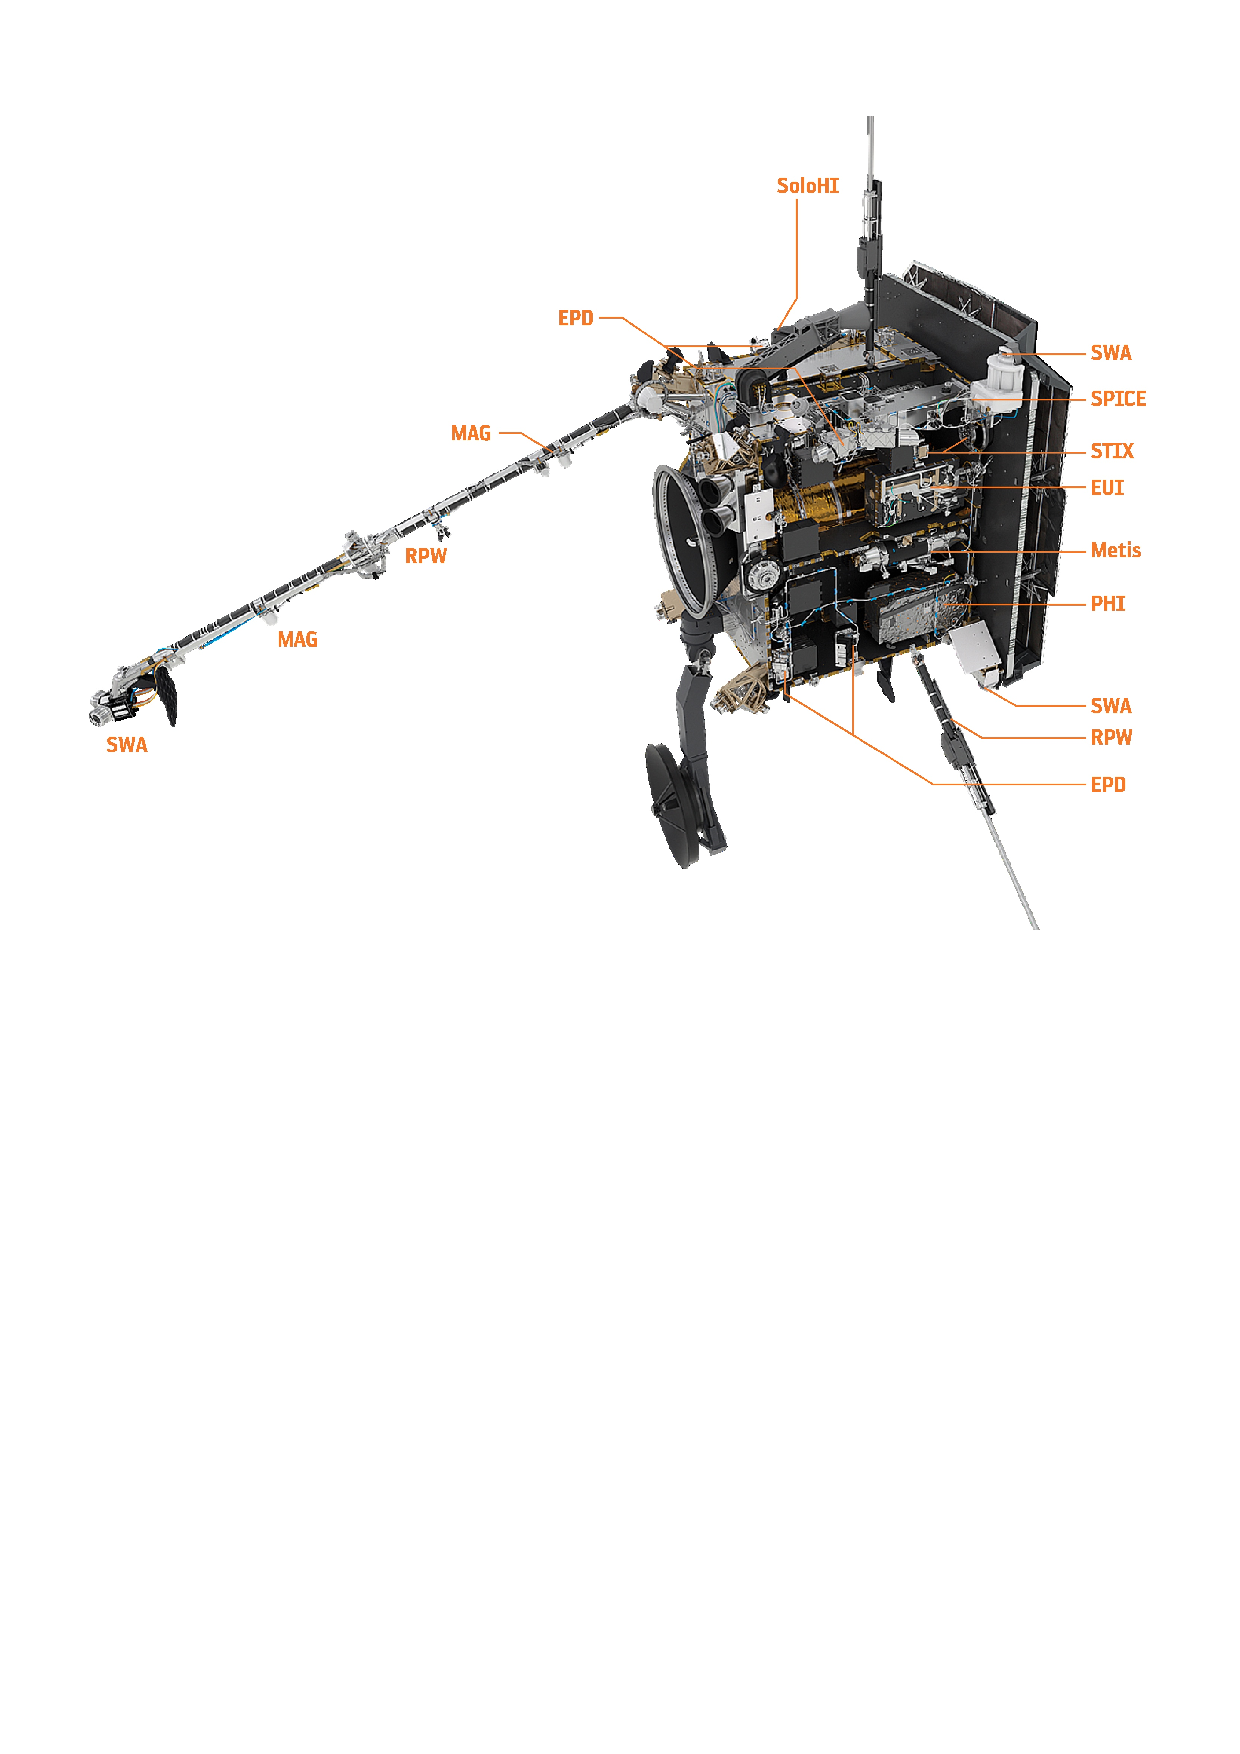
\includegraphics[width=1\linewidth]{figures/instruments.pdf}
    \caption{An image of Solar Orbiter with the -Y side panel removed to indicate the locations of onboard scientific instruments\cite{muller2020}. The boom is shown on the left-hand side of the image. Starting from the tip of the boom, in order of proximity to the spacecraft bus, the indicated instruments are SWA-EAS, MAG-OBS, RPW-SCM, and MAG-IBS\cite{horbury2020}\cite{maksimovic2020}. At the bottom right of the image is SWA-PAS, and at the top right is SWA-HIS\cite{owen2020}. }
    \caption*{Image Source: Müller et al\cite{muller2020}}
    \label{fig: instruments}
\end{figure}
\\

\section{SWA-EAS}

The Solar Wind Analyser suite comprises three in-situ particle sensors, each of which uses the well-established "top hat" electrostatic analyser design\cite{collinson2010}\cite{owen2020} to map incoming particles and their respective velocities/energies across each detector's field of view. The resulting maps give the 3D "velocity distribution functions" (VDFs) for the particles within a given energy range over the measurement period. The three SWA sensors are: 

\begin{enumerate}
    \item The Heavy Ion Sensor (SWA-HIS or HIS), which gives the VDFs of alpha particles and heavier ions in the solar wind to determine their relative charge states and abundances, not only at thermal energies, but also at "suprathermal" energies above the solar wind bulk speed\cite{mason2023}.
    \item The Proton-Alpha Sensor (SWA-PAS or PAS), which gives the VDFs of solar wind protons and alpha particles, mainly at thermal energies.
    \item The Electron Analyser System, which gives the VDFs of solar wind electrons, at thermal and suprathermal energies.
\end{enumerate}

Working in concert, these sensors provide important data about local solar wind plasma to answer some of Solar Orbiter's more specific science questions, such as "What are the source regions of the solar wind and heliospheric magnetic field?", "How do coronal mass ejections (CMEs) evolve through the corona and inner heliosphere?" and "How and where are energetic particles accelerated at the Sun?"\cite{owen2020}. Of the three SWA sensors, this project is most concerned with EAS. 
\\

EAS consists of two radially symmetric electrostatic analysers that inherit several aspects of their design from previous instruments such as the Mars Atmospheric and Volatile EvolutioN (MAVEN) Solar Wind Electron Analyser (SWEA)\cite{mitchell2016} and the Cluster Plasma Electron And Current Experiment (PEACE)\cite{johnstone1997}. The two analysers, also called the "heads" of the instrument\cite{owen2021}, are orthogonal to each other as shown in figure \ref{fig: EAS schematic}. Unlike HIS and PAS, which can afford relatively narrow, sun-pointing fields of view (FOV) of 33° to +66° × ±20° and 24° to +42° × ±22.5° respectively, the EAS sensor heads each observe 360\degree\ of azimuth and ±45\degree\ of elevation in their respective reference frames (see "EAS 1/2 Science Frame" in figure \ref{fig: EAS schematic}), theoretically covering the sky's full 4\(\pi\) steradians between them (e.g. see figure \ref{fig: all bins}). This FOV is required because, in comparison to protons and other ions, electron energies are expected to be much higher than the solar wind plasma bulk velocities. As a result, while protons and other ions are expected to enter their respective sensor primarily from the sun-facing direction, electrons are expected to enter EAS more isotropically\cite{owen2020}. In reality, some of the EAS FOV is always obstructed by a set of support pillars and shielding grid (to avoid spacecraft engine exhaust contamination) around each head, as well as the Solar Orbiter bus high-gain antenna and solar arrays\cite{owen2020}\cite{owen2021}\cite{dickson2024}. To minimise this obstruction, as well as to avoid electrostatic interference from the rest of the spacecraft,  EAS is positioned at the far end of the 4.4m Solar Orbiter instrument boom (see figure \ref{fig: instruments})\cite{owen2020}\cite{olaskoaga2017}.
\\

Ignoring obstructions, solar wind electrons can enter each sensor head from any elevation and azimuth angle in its field of view. As they do so, the electrons fly through an electric field generated by a pair of deflector electrodes at the entrance of the head (subsystems 2b and 2c in figure \ref{fig: EAS cross-section}). The electrodes are charged with positive voltages such that only incoming electrons from a narrow, selected range of elevation angles can continue through the sensor head. Electrons with elevations outside of this range will collide with the sensor walls, evading detection. This range corresponds to a single elevation angle bin. Electrons within the selected elevation range subsequently fly through a pair of hemispherical electrodes (subsystems 3a and 3b in figure \ref{fig: EAS cross-section}), creating their own electric field such that only electrons within a narrow, selected range of velocities/energies can continue to the detector proper, filtering the electron population again. This range corresponds to a single energy bin. If an electron passes through these electron optics, then its trajectory ends when it impinges on a segment of an annular microchannel plate (MCP) corresponding to its azimuthal angle (subsystem 4 in figure \ref{fig: EAS cross-section}). As a result, the incoming electron induces the emission of \(2\times10^{6}-5\times10^{6}\) secondary electrons which collect at the MCP anode, resulting in a characteristic voltage pulse that triggers a detection\cite{owen2020}.
\\

\newpage
\begin{figure}[h!]
    \centering
    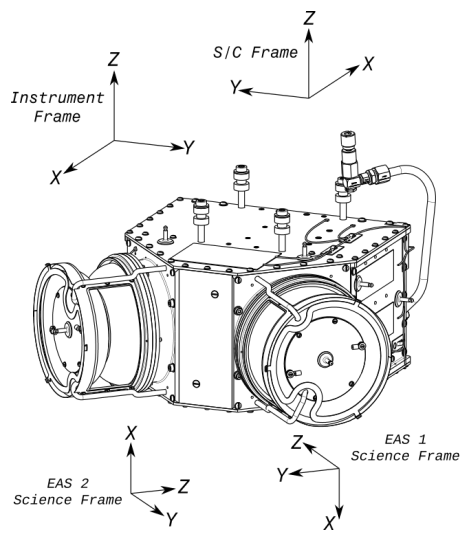
\includegraphics[width=0.75\linewidth]{figures/SWA-EA Sensor Heads.png}
    \caption{An annotated schematic depicting SWA-EAS as it appears on the end of the Solar Orbiter instrument boom (see figure \ref{fig: instruments}), along with the axes of a few salient reference frames\cite{owen2021}. The spacecraft bus is towards the +X direction in the S/C ("spacecraft") frame. The EAS1 sensor head (right) and the EAS2 sensor head (left) can be seen attached to a rectilinear electronics box.}
    \caption*{Image Source: Owen et al\cite{owen2021}}
    \label{fig: EAS schematic}
\end{figure}

During EAS operation, the deflector electrodes sweep through up to 16 elevation bins, sequentially, in the range of ±45\degree. The elevation bins are unequally sized according to a\footnote{due to an error in the EAS data acquisition pipeline which was discovered during this project, solar orbiter has simultaneously used more than one elevation bin table over various periods over the course of its mission.} table of voltages aboard Solar Orbiter, which is designed to account for increasing angular resolution at increasing deflection angles, with bin  widths varying from \(\sim2\degree\) to \(\sim10\degree\). For each elevation bin, the hemispherical electrodes sweep through up to 64 logarithmically-spaced energy bins, sequentially, in the range of \(\sim1\textrm{eV}-5\textrm{keV}\). The full range of 0-360\degree\ of azimuth is split into 32 equally-spaced azimuthal bins, all of which are sampled simultaneously for each combination of elevation and energy. The result is a distribution of solar wind electron energies per solid angle; an electron VDF.
\\

\begin{figure}[h!]
    \centering
    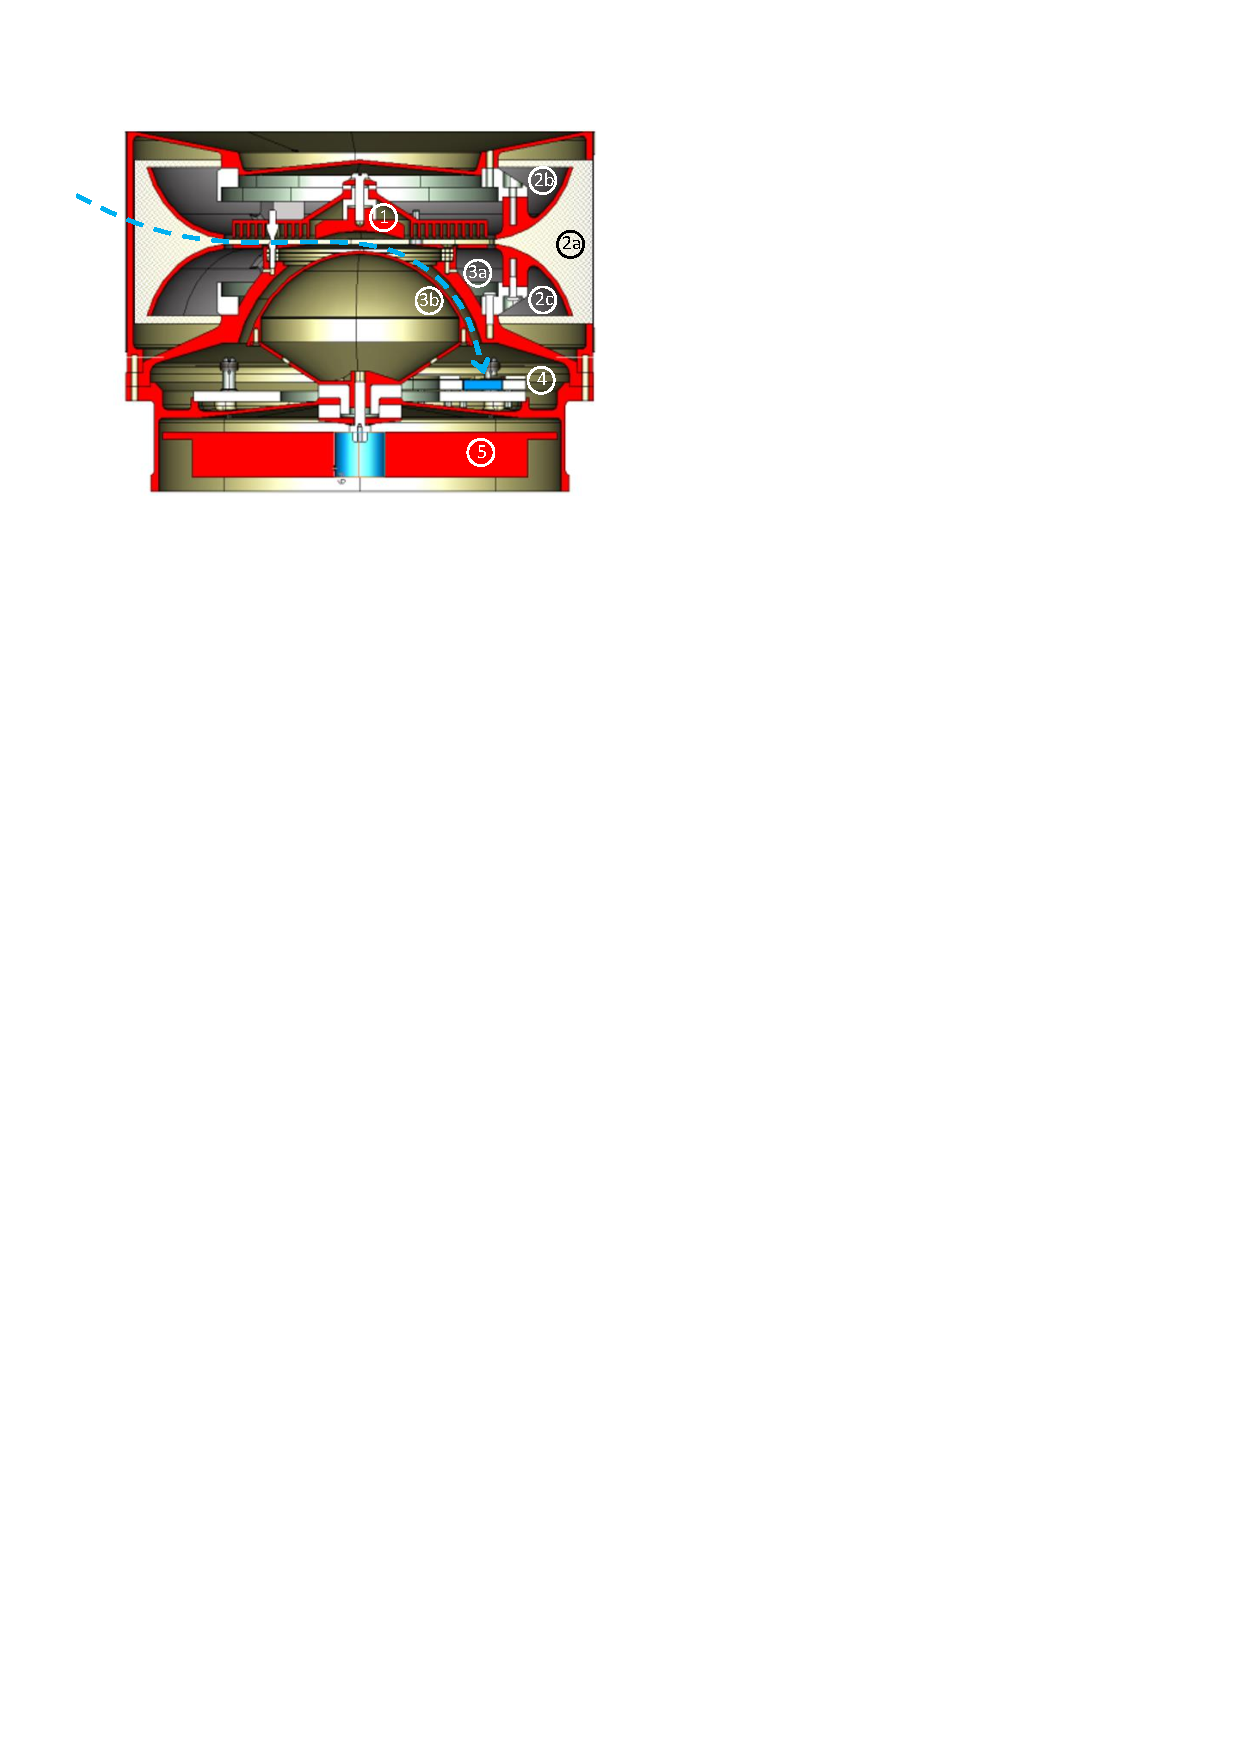
\includegraphics[width=0.75\linewidth]{figures/eas_cross-section.pdf}
    \caption{A diagram showing a cross-section of an EAS sensor head with an example electron trajectory illustrated in blue, and the following annotated subsystems\cite{owen2020}: (1) “top-cap” anode for controlling the geometric factor; (2) (a) sensor shielding grid; (2) (b,c) deflector electrodes for elevation selection; (3) (a,b) hemispherical electrodes for energy selection; (4) MCP subsystem; (5) charge amplifier integrated circuit.}
    \caption*{Image Source: Owen et al\cite{owen2020}}
    \label{fig: EAS cross-section}
\end{figure}

\section{MAG}
The Solar Orbiter magnetometer consists of two three-axis fluxgate magnetometers located on the Solar Orbiter instrument boom. The inboard sensor (MAG-IBS) and outboard sensor (MAG-OBS) respectively (see figure \ref{fig: instruments}).  The two sensors are at different positions along the boom to minimise the risk of magnetic contamination by the rest of Solar Orbiter both by distance attenuation and by subtracting the effect of Solar Orbiter through magnetic gradiometry. The design of MAG borrows heavily from that of previous magnetometers flown on the Cassini\cite{dougherty2004} and Double Star\cite{carr2005}, missions, and forms the basis for future magnetometers on missions including IMAP\cite{mccomas2018}\cite{dickson2024}. The author has previously described the operation of a fluxgate magnetometer as follows\cite{dickson2024}: 

Each magnetometer consists of two orthogonal fluxgate ring-cores (one of which is partially visible in figure \ref{fig: magnetomato}). The fluxgate cores consist of three copper windings; One inner “drive” winding and two outer, orthogonal, “sense” windings. The inner “drive” winding is wound around a ring of magnetically-permeable material which it drives into successive states of oppositely-polarised magnetic saturation at the “drive frequency” through magnetic induction. In an "ideal" environment with no external magnetic field, the magnetic field induced in one half of the ring is designed to perfectly counteract the antisymmetric field induced in the opposite half, resulting a zero magnetic field in the ring overall. However, if an external magnetic field is present and oriented along the plane of the ring, then the drive winding will drive the ring core into magnetic saturation more quickly in the direction parallel to the external magnetic field and more slowly in the direction antiparallel to the external magnetic field. The effect of such an external magnetic field is to temporarily break the symmetry of the induced magnetic field in the ring core, yielding a pulse of non-zero magnetic field which repeats at twice the drive frequency. These pulses of magnetic field density induce a voltage in the outer sense windings depending on their orientation, from which a 2D external magnetic field vector can be recovered. With two orthogonal ring-cores, each fluxgate magnetometer can recover a magnetic field vector in full 3D\cite{horbury2020}\cite{dickson2024}. 
\\

The measured values of the axial components of the external magnetic field vector are known to occasionally “drift” due to imperfections in the magnetometer hardware, leading to offsets that affect magnetic field vector orientation. These offsets are corrected through data processing on the ground and through occasional updates to the software aboard Solar Orbiter\cite{horbury2020}. The central issue in this project is the effect of MAG data inaccuracies such as offset on EAS pitch angle data. 

\begin{figure}[h!]
    \centering
    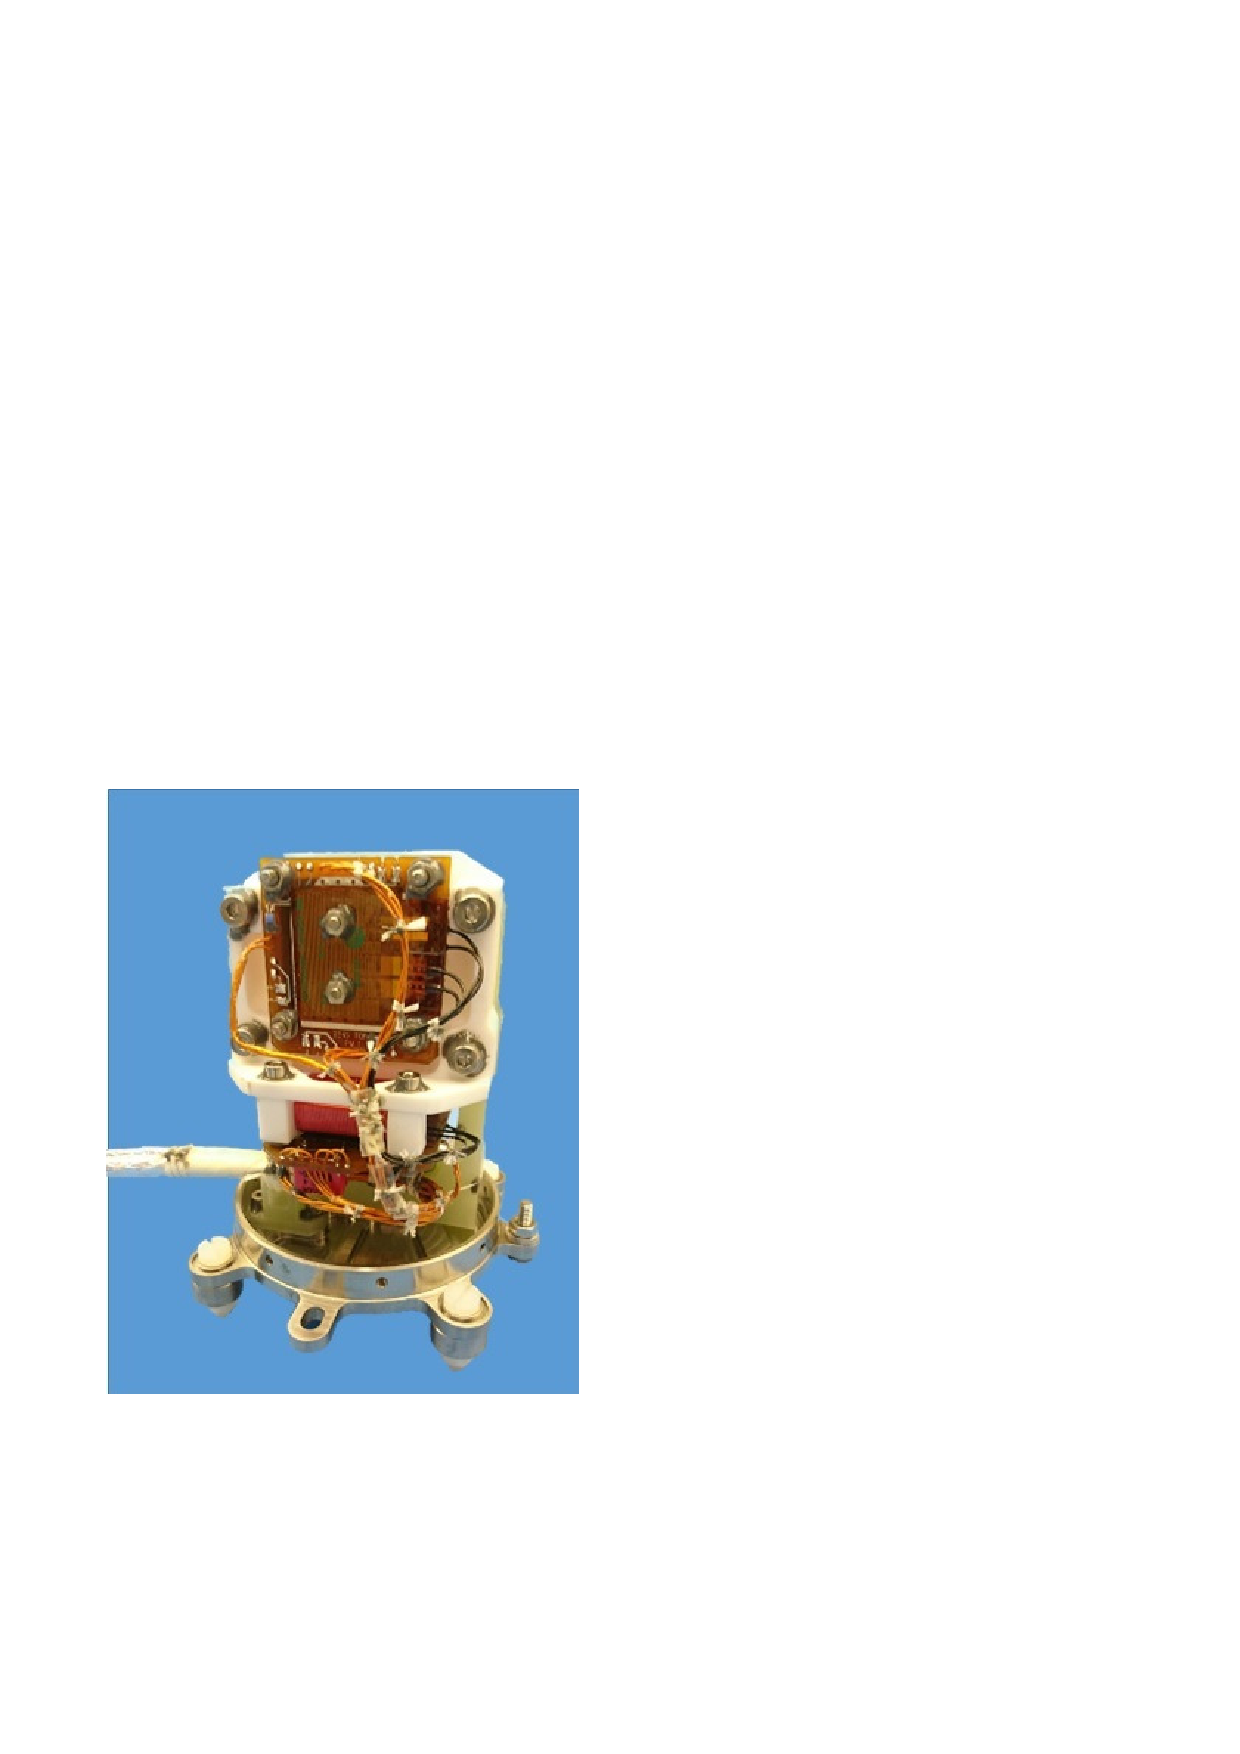
\includegraphics[width=0.5\linewidth]{figures/magnetomato.pdf}
    \caption{An image of one of the Solar Orbiter fluxgate magnetometer sensors as seen in the lab with its protective radiation shield removed\cite{horbury2020}. One ring core with its bright red outermost sense winding can be seen mounted on the underside of a white, ceramic bracket. The other core is unseen, mounted on the other side.}
    \caption*{Image Source: Horbury et al\cite{horbury2020}}
    \label{fig: magnetomato}
\end{figure}

\section{EAS Pitch Angle Distributions} \label{EAS PAD}
A particle's pitch angle, often denoted \(\alpha\), is defined as the angle between the particle's velocity vector \(v\) and the local magnetic field vector \(B\) and is given by

\[\alpha=\textrm{tan}^{-1}(\frac{v_\perp}{v_\parallel})\]

Where \(v_\parallel\) and \(v_\perp\) are the particle's velocity components parallel and perpendicular to \(B\) respectively\cite{pilipp1987}. Analysis of electron pitch angle distributions (PADs) has revealed distinct electron populations in the solar wind. Some populations are able to collide amongst themselves, resulting in a "thermal" distribution with mainly isotropic pitch angles that  can be modeled, to within a close approximation, by a Maxwell-Boltzmann distribution. These represent the "bulk" of the electron plasma. Other populations are far more anisotropic, forming narrow electron beams with pitch angles that may be field-aligned, making up the so-called  electron "strahl". These anisotropic electrons are less likely to collide with eachother, which would have the effect of distributing their trajectories more randomly\cite{pilipp1987}\cite{marsch2006}.
\\

\begin{figure}[h!]
    \centering
    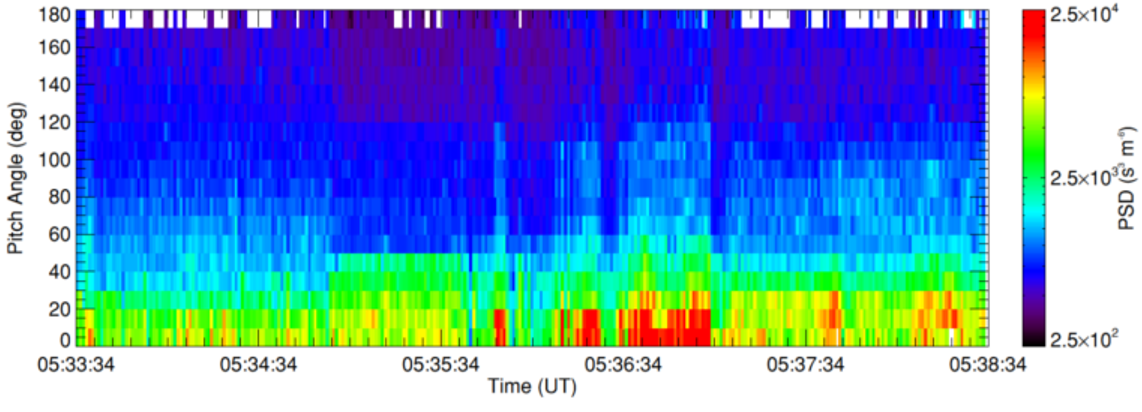
\includegraphics[width=1\linewidth]{figures/PADexample.png}
    \caption{Pitch angle data recorded by Solar Orbiter SWA-EAS in Burst Mode over 5 minutes on 26th June 2020\cite{owen2021}. Electron counts are plotted as a PSD. Time is plotted in Universal Time. Electron pitch angle is plotted in degrees.}
    \caption*{Image Source: Owen et al\cite{owen2021}}
    \label{PAD example}
\end{figure}

An example PAD generated using Solar Orbiter SWA-EAS data is shown in figure \ref{PAD example}\cite{owen2021}. Here, the concentration of electrons is shown as power spectral density (PSD) in colours from black (fewest electrons) to red (most electrons)\footnote{White pitch angle bins on this plot represent missing data, related to each PAD's completeness score, which will be important later.}. There is a different PAD at every 1/8th-second time step (corresponding to EAS Burst Mode; see below). Notice that, for each time step, only pitch angles are shown from 0\degree\ to 180\degree\. It may seem that a full map of the sky would be required to fully capture electron concentrations at different phase angles about the local magnetic field at a given pitch angle, implying \textit{two} angles in spherical coordinates for every time step. However, near this time resolution, it is expected that any instantaneous in-homogeneities in electron concentration at different phase angles about the local magnetic field will disappear too quickly to discern, such that the concentration at all phase angles for a given pitch angle can be assumed to be uniform; in a state of so-called "gyrotropy"\cite{owen2021}. This is expected to be a safe assumption at this timescale\cite{vocks2012}\cite{spinnangr2022}\cite{owen2021}. This can be understood because the expected electron gyroperiod in the solar wind at \(\sim\)1AU is much shorter than the 1/8th-second timescale. Assuming magnetic field strength \(B\approx1\textrm{nT}\), then the electron gyrofrequency \(\omega_{e}\) is  given by 

\[\omega_{e}=\frac{eB}{m_{e}}=\frac{e\times10^{-9}}{m_{e}}\approx176\textrm{ rad/s}\]

where \(m_{e}\) is the electron mass. The corresponding gyration frequency is therefore \(\omega/2\pi\approx28.0\textrm{/s}>>8\textrm{/s}\). Therefore, if this is a realistic estimate, then over a single 1/8th-second measurement, any electron agyrotropy is expected to be thoroughly averaged and rendered indiscernible. Lu et al 2020 has similarly supported the assumption of  gyrotropy when using 1/4th-second time steps in 2D particle-in-cell simulations of magnetic reconnection at earth, on the basis that the local electron gyroradius should be comparable in size to the local plasma ion skin depth - should this be analogous to the EAS environment with the solar wind's plasma parameters to within an order of magnitude, then the assumption of gyrotropy for EAS ought to be safe\cite{lu2020}\cite{lu2019}.
\\

The PAD in figure \ref{PAD example} was taken while EAS was operating in "Burst Mode", which differs from the more typical "Normal Mode" in that it generates PADs \(\sim8\times\) faster. A description of Normal Mode and Burst Mode PAD determination follows.



\subsection{EAS Normal Mode} \label{EAS Normal Mode}

Most EAS data are collected in normal mode, where all 64 energy bins, 16 elevation bins, and 32 azimuth bins are sampled, yielding as close to a full-sky VDF as possible. Cycling through all these bins in sequence takes approximately 1s, yielding Normal Mode data at a data rate of 1Hz. The pipeline involved in acquiring a VDF and a subsequent PAD in Normal Mode can be summarised as follows\cite{owen2020}:

\begin{enumerate}
    \item Acquire a full-sky EAS VDF with 64 energy bins \(\times\) 16 elevation bin \(\times\) 32 azimuth bins at 1Hz,
    \item Acquire a MAG vector at 1Hz,
    \item Downlink EAS VDF and MAG vector to ground,
    \item Post-process MAG vector on ground, applying any necessary corrections,
    \item Combine EAS VDF and MAG vector to yield a PAD.
\end{enumerate}

For a more detailed description, consider figure \ref{fig: all bins}. This figure shows the combined elevation and azimuth bin "pixels" available to each EAS sensor head (EAS1 in blue and EAS2 in red) projected on to a map of the full sky in spherical, spacecraft reference frame (SRF) coordinates where [0,0] points directly away from the sun, and +90\degree\ elevation points out of the ecliptic plane. This amounts to a total of \(16\time32=512\) pixels per head. In normal mode, an EAS head first samples electrons from each of the pixel in its FOV. Simultaneously, MAG samples the local 3D magnetic field vector in its own Burst Mode (128Hz) or Normal Mode (8Hz)\cite{horbury2020}. Now, consider figure \ref{fig: normal - full contours}, where a magnetic field vector from the same period as the 1s PAD is superimposed onto a projection of the EAS1 bins in SRF coordinates. Here, the green diamond represents the vector parallel to the magnetic field (i.e. the B-vector itself), and the green square represents the antiparallel vector. Surrounding the parallel vector are various contours of constant pitch angle at every 15\degree\ in the range 0\degree-180\degree. To aid explanation, let the vectors in figure \ref{fig: normal - full contours} represent the ground magnetic field post-processing\footnote{In reality, this vector was taken from data from the archive corresponding to the unprocessed magnetic field transmitted over the S20 data link in EAS Burst Mode, as will be explained later. Nonetheless, it serves as an analogy for this explanation.}. In this case, wherever an EAS pixel is crossed by a pitch angle contour, that pixel has sampled electrons with the contour's pitch angle. Calculating the pitch angle for every pixel therefore yields a full-sky PAD.

\begin{figure}[h!]
    \centering
    \centerfloat
    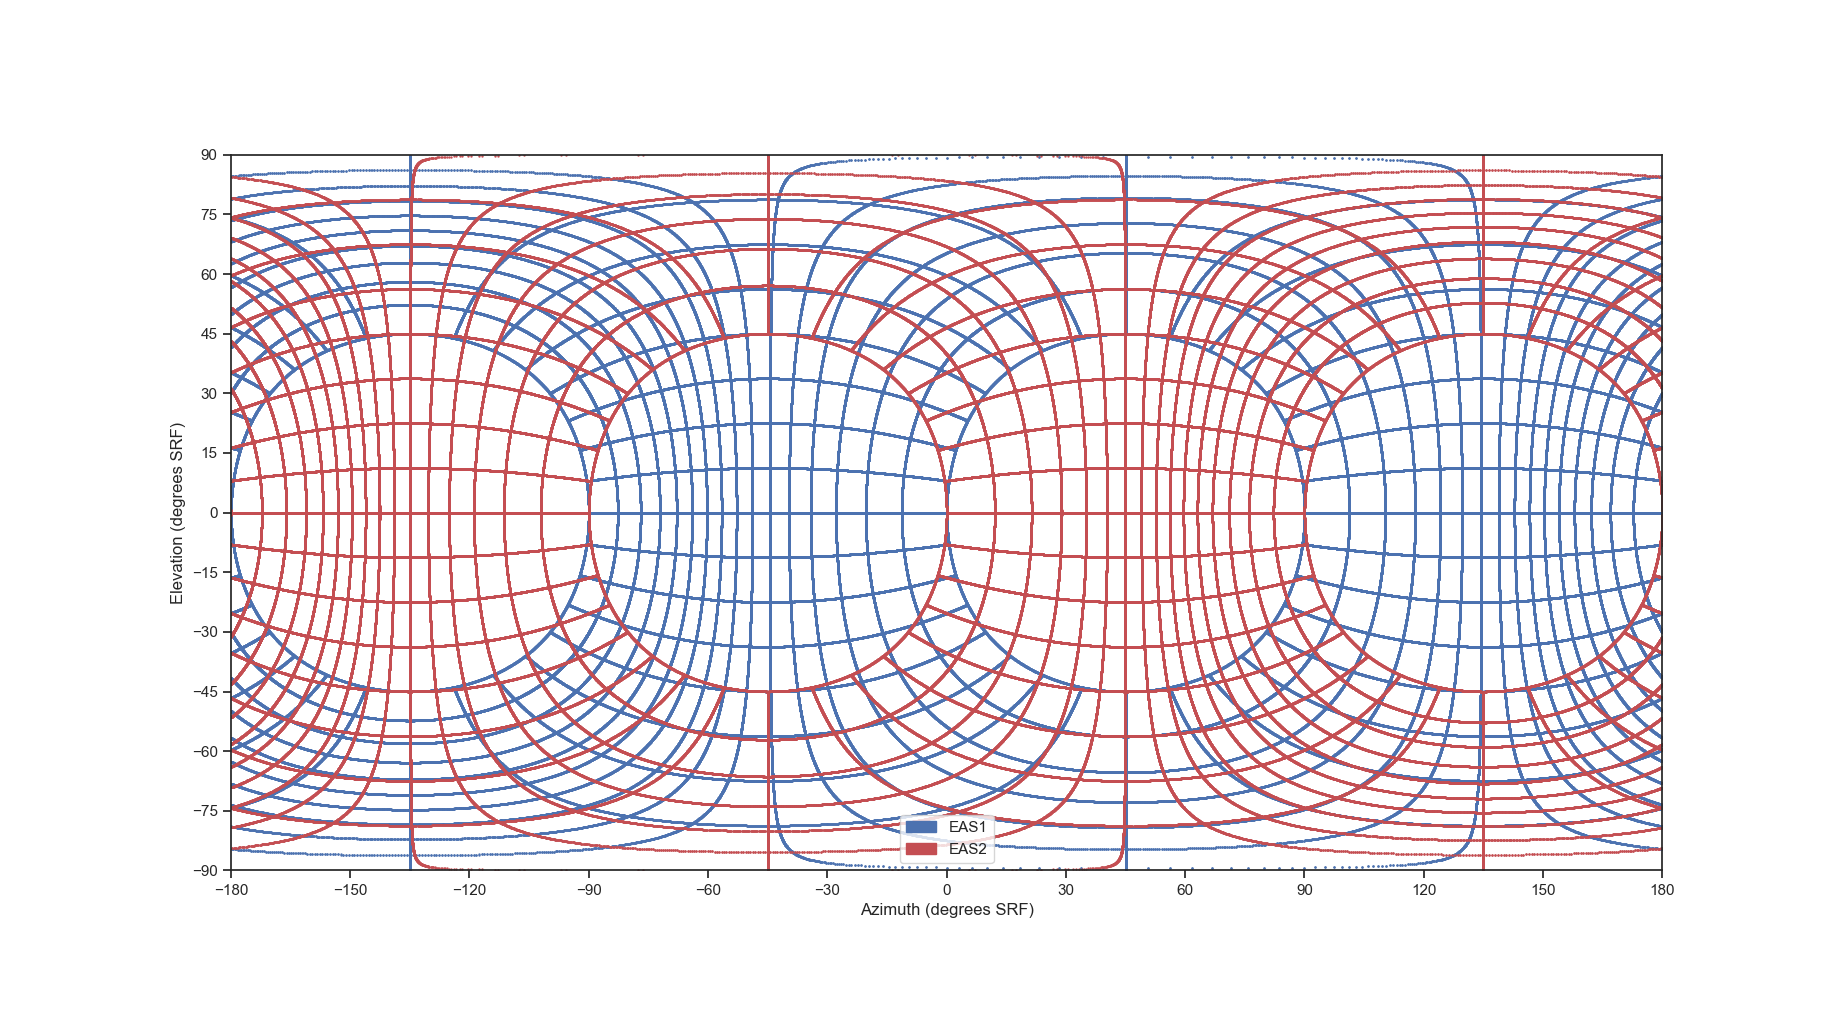
\includegraphics[width=1.3\linewidth]{figures/all bins.png}
    \caption{A plot  of EAS1 (blue) and EAS2 (red) elevation and azimuth bins projected onto the sky in spherical spacecraft reference frame (SRF) coordinates. Note that "elevation" and "azimuth" as labeled in the axes refer to the coordinates in SRF; \textit{not} the elevation/azimuth in the sensor head frames (e.g. figure \ref{fig: EAS schematic}). Note also that between EAS1 and EAS2, it is possible to cover the entire sky with some overlap.}
    \caption*{Image Source: Author's own work}
    \label{fig: all bins}
\end{figure}

\begin{figure}[h!]
    \centering
    \centerfloat
    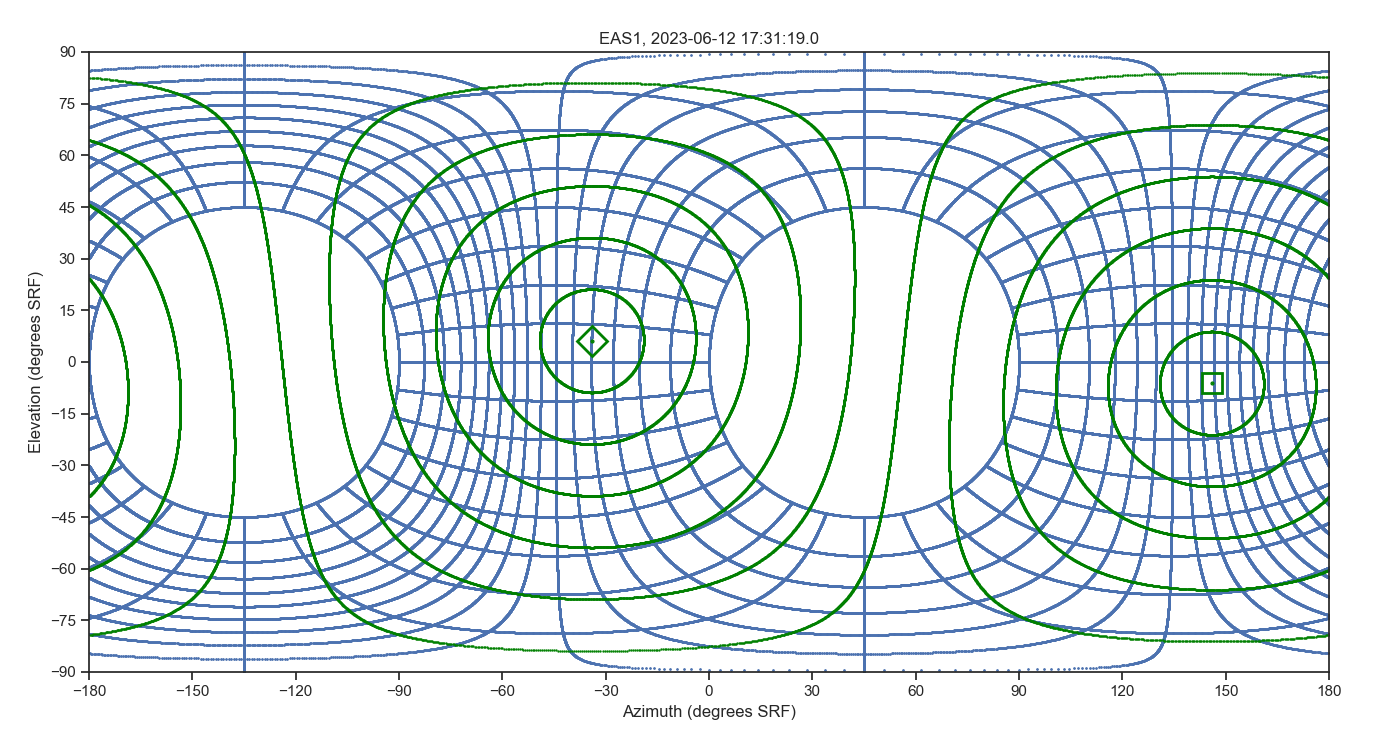
\includegraphics[width=1.05\linewidth]{figures/fullcontours_justeas_noselection.png}
    \caption{Another plot of projected EAS1 elevation and azimuth bins in SRF with an "eas used" magnetic field vector overlay. The point parallel to the vector is indicated by the green diamond, and the point antiparallel to the vector is indicated by the green square. The green contours represent pitch angles of 15\degree, 30\degree, 45\degree, 90\degree, 105\degree, 120\degree, 135\degree, 150\degree, and 165\degree. Vector data are taken from the Solar Orbiter Archive. }
    \caption*{Image Source: Author's own work}
    \label{fig: normal - full contours}
\end{figure}


\newpage
\subsection{EAS Burst Mode} \label{EAS Burst Mode}

EAS Burst Mode data are typically collected over periods of \(\sim5-15\)minutes, once per day. Compared to Normal Mode, full Burst Mode PADs can be acquired after sampling only 2 of the 16 elevation bins in the sky, leading to a theoretical eightfold improvement in data rate (8Hz at \(\sim0.125\)s/sample). The Burst Mode PAD pipeline can be summarised as follows\cite{owen2021}:

\begin{enumerate}
    \item Acquire a MAG vector at 8Hz,
    \item Transmit the MAG vector directly to EAS via the onboard "S20" data link,
    \item Select the EAS head that has the MAG vector closest to the center of its FOV,
    \item For that head, select the \textbf{2} elevation bins that contain the parallel and antiparallel MAG vector in their respective FOVs,
    \item Acquire a partial-sky VDF with 64 energy bins \(\times\) 2 selected elevation bins \(\times\) 32 azimuth bins at 8Hz,
    \item Downlink EAS VDF to ground,
    \item Re-bin EAS VDF on ground, yielding a full PAD.
\end{enumerate}

\begin{figure}
    \centering
    \centerfloat
    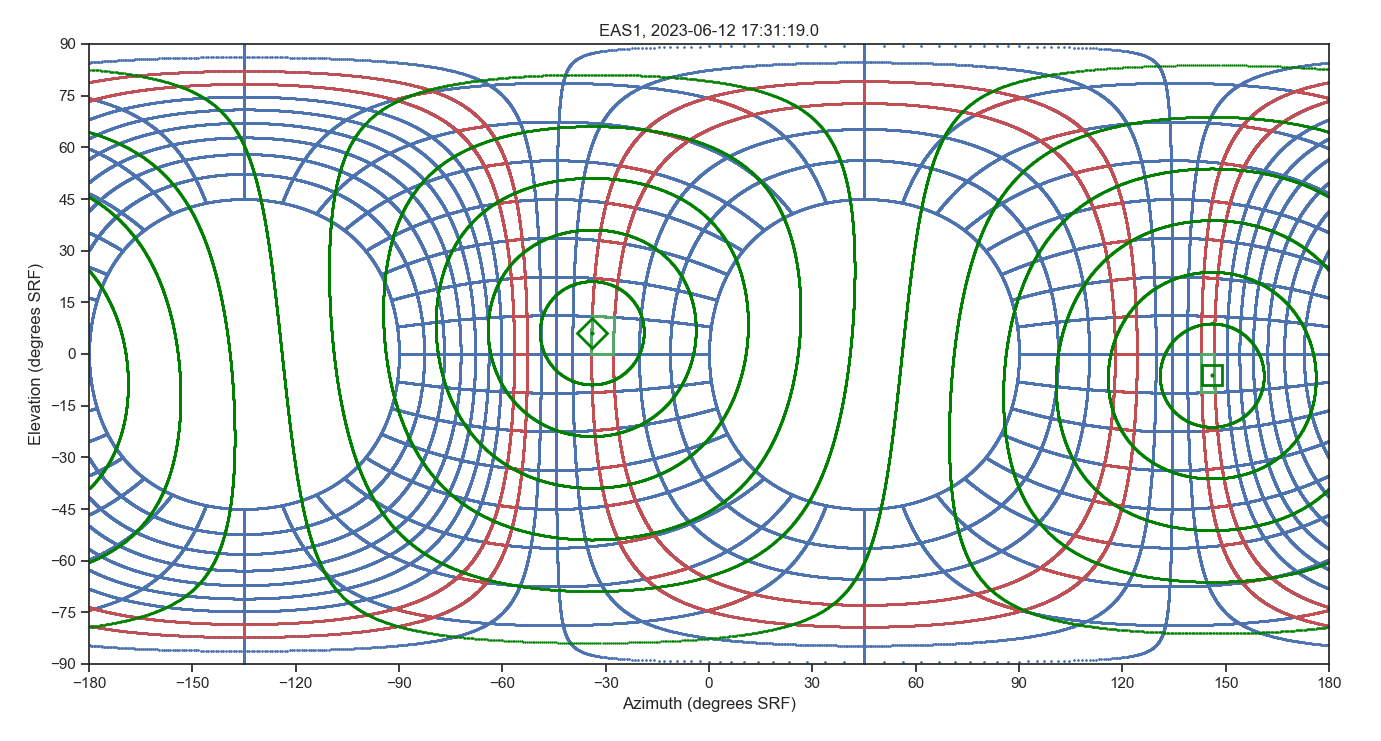
\includegraphics[width=1.05\linewidth]{figures/fullcontours_justeas_yesselection.png}
    \caption{A similar plot to figure \ref{fig: normal - full contours}. Additionally, the bands of EAS1 elevation bins containing the parallel and antiparallel magnetic field vectors are highlighted in red, and the elevation and azimuth pixels containing the same vectors are highlighted in green. Vector data are taken from the Solar Orbiter Archive. }
    \caption*{Image Source: Author's own work}
    \label{fig: normal - full contours + selection}
\end{figure}

For a more detailed description, consider figure \ref{fig: normal - full contours + selection}. This figure shows the same bins, vectors, and pitch angle contours as figure \ref{fig: normal - full contours}, but the bands of elevation bins containing the parallel and antiparallel magnetic field vectors are highlighted in red, and the pixels containing the parallel and antiparallel magnetic field vectors are highlighted in green. Note that each elevation band is separated into azimuthal bins. Within the elevation band containing the parallel vector, as angular distance increases from the azimuthal bin/pixel containing the vector, successive azimuthal bins are crossed by higher and higher pitch angles, culminating in an angle \(\alpha\geq90\degree\). Conversely, as angular distance increases from the azimuthal bin containing the antiparallel magnetic field vector, successive azimuthal bins are crossed by lower and lower pitch angles, culminating in an angle \(\alpha\leq90\degree\). For the sensor head containing the magnetic field vector in its FOV, the geometry of the sensor heads guarantees that this is always true\cite{owen2021}; the two opposite sides of a hypothetical elevation bin at 0\degree\ elevation would reach a maximum of \(\sim180\degree\) apart, and the opposite sides of an elevation bin at \(\pm45\degree\) would reach a minimum of \(\sim90\degree\) apart. Therefore, by "steering" EAS to sample each azimuthal bin across only the two highlighted elevation bands, it is possible to sample electrons with a full range of 0\degree-180\degree\ pitch angles. With the assumption of gyrotropy, this represents a full PAD (e.g. figure \ref{PAD example}). Since the 32 azimuth bins at each elevation are sampled simultaneously, this costs no additional time, resulting in an eight-fold sample time reduction.
\\

To sample only the elevation bins containing the parallel and antiparallel magnetic field vector, EAS must first be told the orientation of the magnetic field. On Solar Orbiter, this is communicated via the "S20 inter-instrument communications link" which is transmitted by the MAG Instrument Control Unit (MAG-ICU) and received by the SWA Data Processing Unit (SWA-DPU)\cite{owen2021}\cite{owen2020}\cite{horbury2020}. Once received, SWA-DPU must select the EAS head that has the magnetic field closest to the center of its FOV, which is equivalent to finding the smallest angle between the vector and the sensor head aperture center-plane\cite{owen2021}.
\\

While Burst Mode boasts superior time resolution, it is also vulnerable to errors that Normal Mode avoids. By virtue of the fact that Burst Mode uses MAG data transmitted directly over the S20 data link, it therefore also circumvents post-processing of magnetic field data on the ground. Errors that may result in a discrepancy between the vectors used to "steer" EAS and the "true" vectors available on the ground include: 
\begin{itemize}
    \item Un-calibrated offset drift in MAG measurement axes\cite{owen2021}\cite{horbury2020}. 
    \item Data latency in the S20 inter-instrument link itself, which may be inherent and/or exaggerated  by periods  of heavy data traffic\cite{owen2021}.
\end{itemize}

When errors like these cause EAS to select to incorrect elevation and azimuth bins in Burst Mode, this can lead to missing and mislabelled PAD data. The next chapter describes the methods applied to determine the impact of these errors on Burst Mode PAD accuracy and completeness and to encapsulate some of that impact in the form of a "completeness score".


\chapter{Methods}
\label{chapterlabel2}

To determine the accuracy and completeness of Burst Mode data collection it is useful to compare 3D magnetic field vectors used to steer EAS in Burst Mode (which will be called "\(B_{EAS}\)") to corresponding examples of the ground-calibrated and "true" magnetic field vectors (which will be called "\(B_{MAG}\)"). That requires data.
\\

\section{Data Access}
The online Solar Orbiter Archive (SOAR) regularly publishes science data at various processing levels from Solar Orbiter instruments including MAG and EAS where they can be accessed by the public\cite{soar}. Most science data,including MAG vector time series and EAS Burst Mode PADs, are published in CDF, which is a "Self-describing data format for the storage of scalar and multidimensional data in a platform- and discipline-independent way"\cite{cdf}. Developed by NASA Goddard Space Flight Center, CDF is close to an industry-standard data format used frequently in NASA/ESA projects\cite{horbury2020}. CDF files accommodate data fields for different variables including science data and associated metadata/support data, along with various tags and descriptions. The primary data and metadata in a CDF file can be previewed via the SOAR interface, and accessed/manipulated through freely available libraries built for Python and MATLAB\cite{cdf}.
\\

EAS and MAG data products are published to SOAR at various levels of usability; some are "raw" data directly from the instrument, and others are thoroughly processed and ready to be used in conventional, publishable research\cite{horbury2020}\cite{owen2020}\cite{zouganelis2020}. The author has previously described the data levels for EAS and MAG as follows\cite{dickson2024}:
\\

\textbf{EAS Data Levels\cite{owen2020}:}
\begin{itemize}
    \item \textbf{Level 0:} Uncalibrated CCSDS\cite{CCSDS_Standards_2022} binary data packets.
    \item \textbf{Level 1:} Uncalibrated electron count data converted to CDF in Burst Mode and Normal Mode. At this level, the MAG vectors used to steer EAS during Burst Mode (\(B_{EAS}\)) are also included.
    \item \textbf{Level 2:} Calibrated electron count data including Burst Mode PADs, but excluding \(B_{EAS}\).
    \item \textbf{Level 3:} A subset of level 2 data with additional processing.
\end{itemize}
\\

\textbf{MAG Data Levels\cite{horbury2020}:}
\begin{itemize}
    \item \textbf{Level 0:} Uncalibrated binary data.
    \item \textbf{Level 1:} Uncalibrated time series data in nT in each MAG sensor's reference frame.
    \item \textbf{Level 2:} Calibrated time series data in radial-tangent-normal (RTN), and Spacecraft Reference Frame (SRF) coordinates, corrected for offset drift and other inaccuracies, published at various cadences including E8 normal mode (8Hz) and E128 burst mode (128Hz).
    \item \textbf{Level 3:} A subset of level 2 data with additional processing.
\end{itemize}
\\

EAS level 1 Burst Mode CDF files are typically published at a rate between \(\sim\)5min/day and \(\sim\)15min/day. Some of these, published to SOAR under "solo\_L1\_swa-eas-padc\_\textit{YYYYMMdd}T\textit{hhmmss}-\textit{YYYYMMdd}T\textit{hhmmss}\_V01.cdf" are packaged with \(B_{EAS}\) as metadata in the form of normalised vectors in the SRF frame under the variable "SWA\_EAS\_MagDataUsed". 

MAG level 2 SRF CDF files, published to SOAR under "solo\_L2\_mag-srf-normal\_\textit{YYYYMMdd}\_V01", contain many hour's worth of ground-calibrated 8Hz MAG data per day (i.e. \(B_{MAG}\)), all in the same reference frame as \(B_{EAS}\) at the time of publishing (SRF), under the variable "B\_SRF".
\\

The desired CDFs were downloaded and manipulated using Python scripts with the \textit{pycdf} package in the Spacepy library. Spacepy is "a package for Python, targeted at the space sciences, that aims to make basic data analysis, modeling and visualization easier"\cite{niehof2022spacepy}. Pycdf allows individual CDF data fields to easily be referenced by name and converted to \textit{numpy} arrays as required\cite{harris2020numpy}.

\section{Time Axis Cropping}
\(B_{EAS}\) and \(B_{MAG}\) can be plotted together to yield an initial estimate of the discrepancies between them, but their respective time series are uploaded to SOAR with notably different durations (5-15 minutes vs several hours). This makes it difficult to compare one time series to the other numerically using Python, unless the longer time series is first cropped.  Several algorithms were implemented to crop magnetic field time series. Initial attempts involved simply cropping the start and end of the longer series  (\(B_{MAG}\)) to the shorter series (\(B_{EAS}\)). While this worked for some EAS CDFs (e.g. solo\_L1\_swa-eas-padc\_20231105T172733-20231105T174232\_V01.cdf and solo\_L1\_swa-eas-padc\_20230831T172734-20230831T173233\_V01.cdf), this could not be generalised to some older CDFs (e.g. solo\_L1\_swa-eas-padc\_20200624T053335-20200624T063334\_V01.cdf and solo\_L1\_swa-eas-padc\_20221201T052733-20221201T220001\_V01.cdf) whose time series began in the 1700s for the first few data points. At the time of writing, this is not signposted on SOAR, and these data points were not cropped by this algorithm. In the interest of generality, the ultimate cropping algorithm was adapted to read the timestamps in the titles of the CDFs as the start and end times to crop to, and both time series were cropped to those times instead. At present, this leads to a small amount of missing data near the start/end of a time series because the CDF filenames do not include millisecond accuracy, but this is easily fixed in the future.
\\

Once the desired start and end of an arbitrary time series are defined, an algorithm was implemented to efficiently identify the data points in that time series that should be cropped. The algorithm is summarised here:
\begin{enumerate}
    \item Determine if the time series overlaps with the desired start and stop times by performing two comparisons.
    \item If the time series overlap, then take the time in the middle of the series and determine if it is before or after the start time. 
    \item Whichever region the start time lies in, divide that region in half again and repeat N-2 times where N is the number of search divisions (typically, N=5. More divisions show diminishing returns in efficiency).
    \item Once the number of divisions has been reached, loop through the time series until the time is greater than or equal to the start time. Crop when you find the start time.
    \item Starting from the start time, loop through the time series again until the time is greater than or equal to the stop time, and then crop again.
\end{enumerate}

Implementations of this algorithm without step 6 had to loop through comparisons with every data point in a \(B_{MAG}\) time array that was several hours long. Given that the time values are saved as relatively inefficient \textit{datetime.datetime()} values, these comparisons often took \(>\)20s to complete. The inclusion of step 6 reduced this time to \(<\)2s. The core algorithm is written in Python as follows:
\\

\lstset{basicstyle=\tiny, style=myCustomMatlabStyle}
\begin{lstlisting}[language=Python]
time_index = 0
for i in range(1,searchdivisions+1):
    time_index += int(length/2**i)*(time_array[time_index+int(length/2**i)] < time_reference)
while (time_array[time_index] < time_reference) and (time_index < length-1):
    time_index += 1
\end{lstlisting}
\\

where \textit{time\_array} is the array of time values being cropped, \textit{time\_reference} is the time in \textit{time\_array} to crop at, \textit{time\_index} is an index in \textit{time\_array} within one index of \textit{time\_reference}, and \textit{length} is the length of \textit{time\_array}.
\\

As-implemented, this algorithm sometimes leads to "off by one" errors in time series length. This may be the result of comparing time series that are not using the exact same time grid, because \(B_{EAS}\) is synchronised to EAS Burst Mode time and \(B_{MAG}\) is synchronised to MAG time. In response, if \(B_{EAS}\) and \(B_{MAG}\) are not the same length after cropping, then the longer of the two time series is cropped to the shorter starting with the last data point. This may lead to some artificial time delay between the two time series.

\section{Coordinate Systems} \label{coordinate systems}

\begin{figure}[h!]
    \centering
    \centerfloat
    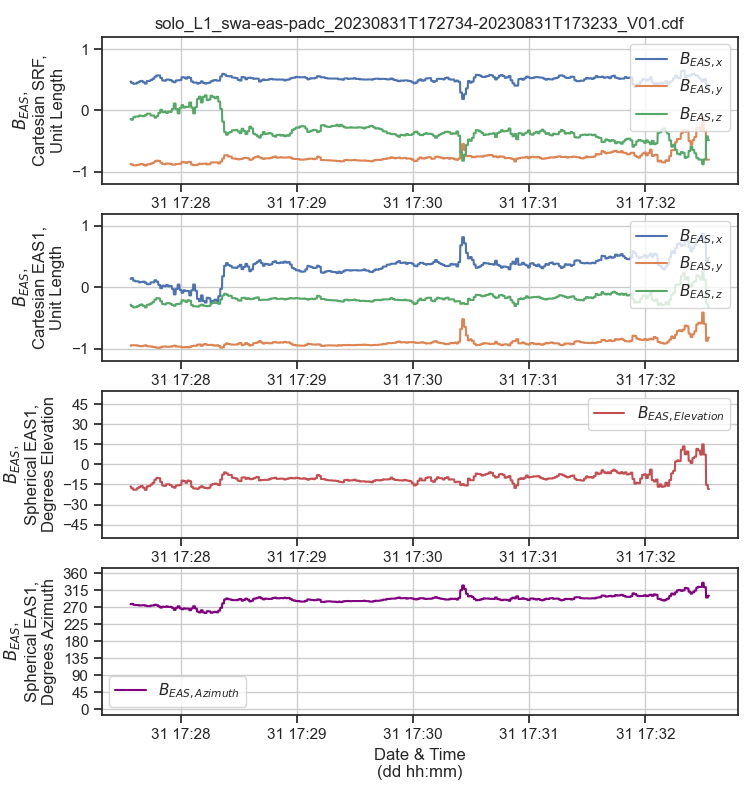
\includegraphics[width=1.05\linewidth]{figures/Transformation Example.png}
    \caption{Example \(B_{EAS}\) data from 31st August 2023. Top panel: Default cartesian \(B_{EAS}\) in SRF frame. 2nd panel: Cartesian \(B_{EAS}\) in EAS1 frame. 3rd panel: Elevation for spherical \(B_{EAS}\) in EAS1 frame. bottom panel: Azimuth for spherical \(B_{EAS}\) in EAS1 frame. The radius in spherical coordinates is not shown because all time series vectors are of length unity.}
    \caption*{Image Source: Author's own work}
    \label{fig: trans example}
\end{figure}

\(B_{EAS}\) and \(B_{MAG}\) are both acquired from SOAR in cartesian SRF coordinates. This is contrasted with data in cartesian radial-tangent-normal (RTN) coordinates (which are also provided for MAG\cite{soar}), where the "x-axis" is oriented radially away from the sun, the "z-axis" is oriented towards the north celestial pole, and the "y-axis" is tangent to a prograde orbit in the plane of the ecliptic, completing the triad. SRF coordinates are thought to correspond to the "S/C Frame" shown in figure \ref{fig: EAS schematic}, which is approximately equivalent to RTN coordinates with the "x and y" axes inverted. However, this equivalence depends on Solar Orbiter's pointing accuracy, meaning that transformations between rigidly-coupled onboard reference frames (e.g. SRF and the EAS Instrument frame in figure \ref{fig: EAS schematic}) are generally expected to be more consistent than transformations between onboard reference frames and celestial reference frames such as RTN\cite{erofeev2019}.
\\

To determine the effect of \(B_{EAS}\) and \(B_{MAG}\) on EAS elevation/azimuth binning, these time series had to be converted from cartesian SRF coordinates to spherical EAS1/EAS2 coordinates in terms of radius and elevation and azimuth angles, where the head should be chosen such that \(B_{EAS}\) and/or \(B_{MAG}\) lie within that head's FOV. This was calculated in the following order: Cartesian SRF \(\rightarrow\) Cartesian EAS1/2 \(\rightarrow\) Spherical EAS1/2. This order was chosen because SOAR provides "EAS\textit{X}\_TO\_SRF" transformation matrices packaged with level 2 EAS data CDF files published under "solo\_L2\_swa-eas\textit{X}-nm3d-dnf\_\textit{YYYYMMdd}T\textit{hhmmss}-\textit{YYYYMMdd}T\textit{hhmmss}\_V01.cdf" where \textit{X} is the EAS head number (1 or 2). Despite being packaged with timestamped CDF files, these transformation matrices do not appear to change over time (nor should they be expected to change over time). The matrices can be trivially inverted to enable a Cartesian SRF \(\rightarrow\) Cartesian EAS1/2 transformation. The default and inverted forms are shown in table \ref{tab: EASX to SRF}, as would be expected geometrically based on figure \ref{fig: EAS schematic}.
\\

\begin{table}[h!]
    \centering
    \(
    \begin{array}{cc}
        \text{EAS1 to SRF} & \text{SRF to EAS1} \\
        \begin{bmatrix}
        0 & -\frac{\sqrt{2}}{2} & +\frac{\sqrt{2}}{2}\\
        0 & +\frac{\sqrt{2}}{2} & +\frac{\sqrt{2}}{2}\\
        -1 & 0 & 0\\
        \end{bmatrix} &
        \begin{bmatrix}
        0 & 0 & -1\\
        -\frac{\sqrt{2}}{2} & +\frac{\sqrt{2}}{2} & 0\\
        +\frac{\sqrt{2}}{2} & +\frac{\sqrt{2}}{2} & 0\\
        \end{bmatrix}
        \\
        \\
        \text{EAS2 to SRF} & \text{SRF to EAS2} \\
        \begin{bmatrix}
        0 & -\frac{\sqrt{2}}{2} & +\frac{\sqrt{2}}{2}\\
        0 & -\frac{\sqrt{2}}{2} & -\frac{\sqrt{2}}{2}\\
        -1 & 0 & 0\\
        \end{bmatrix} &
        \begin{bmatrix}
        0 & 0 & -1\\
        -\frac{\sqrt{2}}{2} & -\frac{\sqrt{2}}{2} & 0\\
        +\frac{\sqrt{2}}{2} & -\frac{\sqrt{2}}{2} & 0\\
        \end{bmatrix}
        \\
        
    \end{array}
    \)\\
    \caption{A table of transformation matrices between SRF and EAS1/2 coordinates in cartesian space. The matrices in the left column were found on SOAR (in reality, \(\pm\sqrt{2}/2\) was approximated as \(\pm0.707\) on SOAR).} 
    \label{tab: EASX to SRF}
\end{table}


Once in the EAS1/2 frame, the Cartesian EAS1/2 \(\rightarrow\) Spherical EAS1/2 transformation was calculated using the \textit{astropy} library for Python; in particular, the \textit{CartesianRepresentation(x,y,z)} object with the \textit{.represent()} method\cite{astropy2013}\cite{astropy2018}\cite{astropy2022}. Figure \ref{fig: trans example} shows an example of normalised \(B_{EAS}\) data from 31st August 2023 is shown at each stage of transformation from unit cartesian SRF to unit spherical coordinates in the EAS1 frame. Since the vector time series is normalised from the start, a time series of the radius in spherical coordinates would be trivial and is omitted from figure \ref{fig: trans example}. In figure \ref{fig: trans example}, the x-axis, y-axis, and z-axis in the top panel (cartesian SRF) appear to align most closely with the z-axis (+ an offset), the y-axis (+ an offset), and the opposite of the x-axis in the 2nd panel (cartesian EAS1) respectively. This is also expected based on the "S/C" and "EAS 1 Science" frames in figure \ref{fig: EAS schematic}, further validating the matrices in table \ref{tab: EASX to SRF}.
\\


\section{Preliminary \(B_{EAS}\)-\(B_{MAG}\) Comparison}
As described in the author's earlier work, a preliminary comparison was performed between \(B_{EAS}\) and \(B_{MAG}\) from a small set of arbitrarily selected periods of Burst Mode data to justify the creation of a completeness score\cite{dickson2024}.
\\

\(B_{EAS}\) time series are stored in EAS burst mode CDF files under "SWA\_EAS\_MagDataUsed" and "EPOCH" respectively. \(B_{MAG}\) time series are stored in MAG SRF normal mode CDF files under "B\_SRF" and "EPOCH" respectively. Each "B\_SRF" vector was normalised before comparison with \(B_{EAS}\). The dot product between \(B_{EAS}\) and \(B_{MAG}\) vectors gives the angular offset between them. This angle was calculated for every vector in the sample of time series, which when plotted for 31st August 2023 yields figure \ref{fig: angle example august}.
\\

\begin{figure}[h!]
    \centering
    \centerfloat
    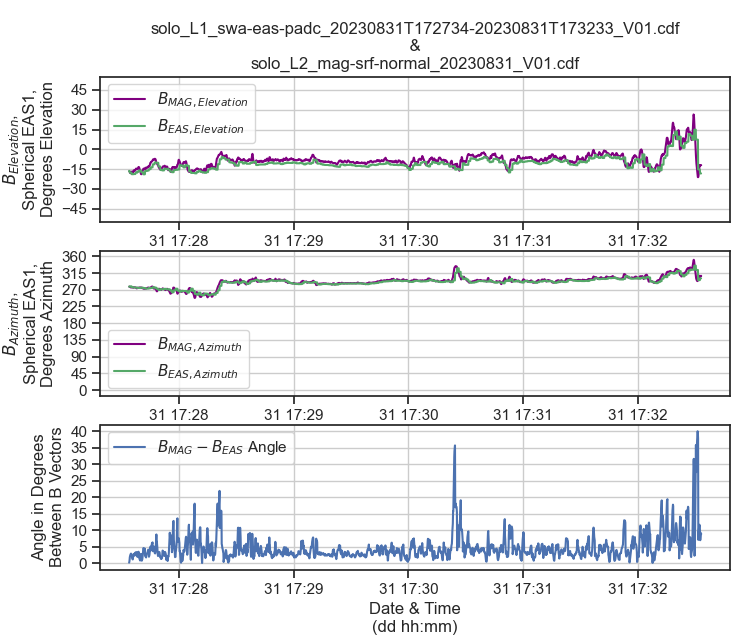
\includegraphics[width=1.05\linewidth]{figures/Angle Example.png}
    \caption{Example \(B_{EAS}\) data from a 5 minute period of EAS Burst Mode on 31st August 2023. Top panel: Elevation for \(B_{EAS}\) and \(B_{MAG}\) in spherical EAS1. Middle panel: Azimuth for \(B_{EAS}\) and \(B_{MAG}\) in spherical EAS1. Bottom panel: Angular difference between \(B_{EAS}\) and \(B_{MAG}\).}
    \caption*{Image Source: Author's own work}
    \label{fig: angle example august}
\end{figure}

\begin{figure}[h!]
    \centering
    \centerfloat
    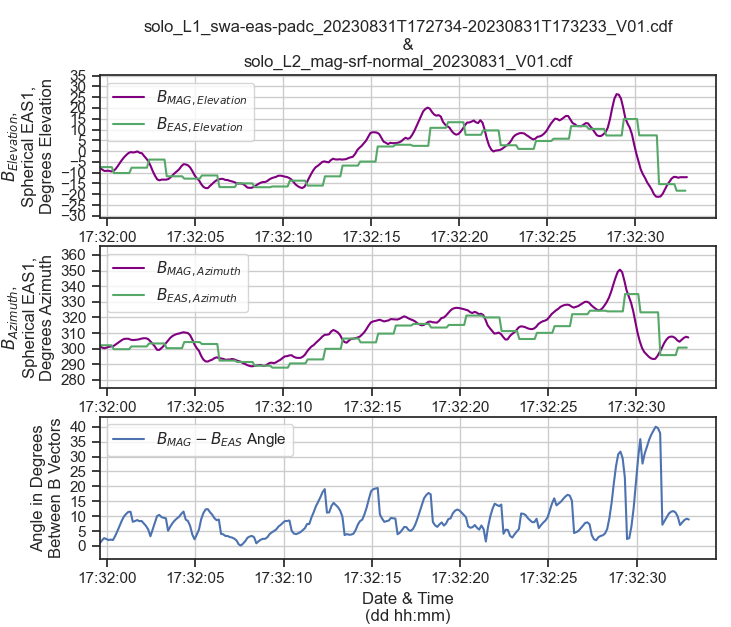
\includegraphics[width=1.05\linewidth]{figures/Angle Example Detail.png}
    \caption{A detailed look at the last \(\sim5\)s of figure \ref{fig: angle example august}. Top panel: Elevation for \(B_{EAS}\) and \(B_{MAG}\) in spherical EAS1. Middle panel: Azimuth for \(B_{EAS}\) and \(B_{MAG}\) in spherical EAS1. Bottom panel: Angular difference between \(B_{EAS}\) and \(B_{MAG}\).}
    \caption*{Image Source: Author's own work}
    \label{fig: angle example detail august}
\end{figure}

By inspection, while relatively good agreement can be seen between \(B_{EAS}\) and \(B_{MAG}\) over large timescale, there are clear discrepancies over short timescales as shown in figure \ref{fig: angle example detail august}. An unexpected observation is that \(B_{EAS}\) has less time resolution than \(B_{MAG}\), appearing only to update at 1Hz. Inspection of the raw "SWA\_EAS\_MagDataUsed" data 
By inspection, while relatively good agreement can be seen between \(B_{EAS}\) and \(B_{MAG}\) over large timescale, there are clear discrepancies over short timescales as shown in figure \ref{fig: angle example detail august}. An unexpected observation is that \(B_{EAS}\) has less time resolution than \(B_{MAG}\), appearing only to update at 1Hz. Inspection of the raw "SWA\_EAS\_MagDataUsed" time series data reveals that while this data array \textit{is} published to SOAR with 8 vectors for every second of "EPOCH" as advertised, these vectors are only updated once per second resulting in 8 identical vectors per second such that the effective cadence is 1Hz. Since these data are packaged in level 1 CDF files, they are expected to represent the true MAG data used to steer EAS, which implies that the alleged 1/8th second resolution of EAS Burst Mode is compromised by a magnetic field vector only updates at 1Hz. This will be a particular source of error during periods of fast-changing magnetic field. This effective 1Hz effect has been observed in other periods of Burst Mode from the sample including 5th November 2023 and 1st January 2023. It is absent from the relatively quiet period on 30th May 2023. Further research is required to determine the cause for this unexpectedly low update cadence.
\\

The highest angular offset in figure \ref{fig: angle example august} is observed to exceed 40\(\degree\), and it exceeds 70\(\degree\) in a different example from 5th November 2023. Otherwise, the offset is near 10\(\degree\) for most of figure \ref{fig: angle example august} and near 3\(\degree\) for a different example from 30th May 2023. Given that an individual EAS sensor head has an elevation FOV of \(\pm45\degree\) (range of 90\(\degree\)) separated into 16 bins of various sizes, the average bin width can be estimated to be \(\frac{90\degree}{16 \textrf{bins}} = 5.625\degree / \textrf{bin}\). The actual bin centers and bin widths for elevation and azimuth are tabulated with level 2 EAS data CDF files alongside the aforementioned transformation matrices. While azimuth bins are identical for both heads, elevation bins are different due to tuning of the EAS electron optics. These tables have been updated over time but remained constant since 17th July 2021. These are included in appendix \ref{appendixlabel1}. The widest angular bin in EAS1 has width \(\pm6.06\degree\). This is well below much of the angular offset observed in the sample, therefore, it is established that \(B_{EAS}\) could cause erroneous Burst Mode steering, which justifies a quality score's development.

\section{Simulating EAS Burst Mode Steering} \label{sim steering}

\begin{figure}[h!]
    \centering
    \centerfloat
    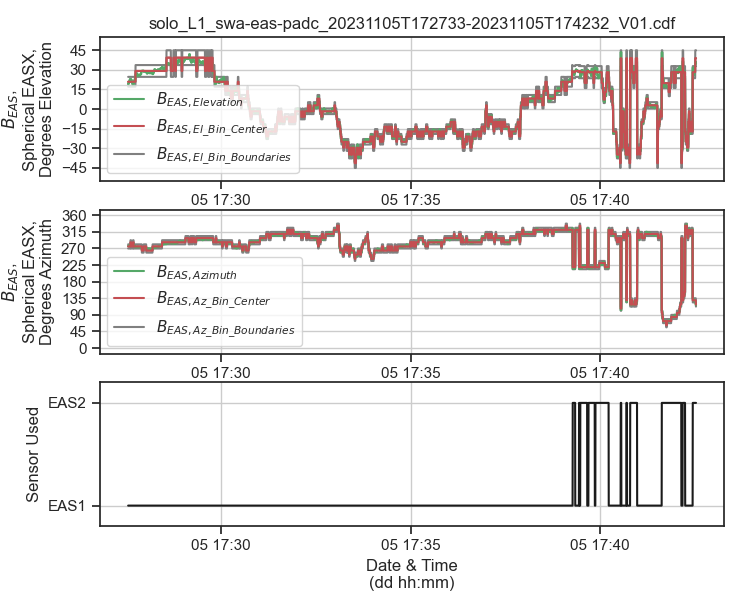
\includegraphics[width=1.05\linewidth]{figures/Steering Example.png}
    \caption{Example \(B_{EAS}\) data from a 15 minute period of EAS Burst Mode on 5th November 2023 showing a simulation of the Burst Mode steering algorithm. The reference frame for the top two panels is labeled "EASX" to indicate that it switches between EAS1 and EAS2 over the 15 minute period depending on \(B_{EAS}\) orientation and resulting head selection. Top panel: Elevation for \(B_{EAS}\) in spherical EASX, along with the centers and upper/lower bounds of the selected elevation bins ("El\_Bin\_Center" and "El\_Bin\_Boundaries" respectively). Middle panel: Azimuth for \(B_{EAS}\) in spherical EASX, along with the centers and upper/lower bounds of the selected azimuth bins ("Az\_Bin\_Center" and "Az\_Bin\_Boundaries" respectively). Bottom panel: The selected head over time.}
    \caption*{Image Source: Author's own work}
    \label{fig: steering example november}
\end{figure}

\begin{figure}[h!]
    \centering
    \centerfloat
    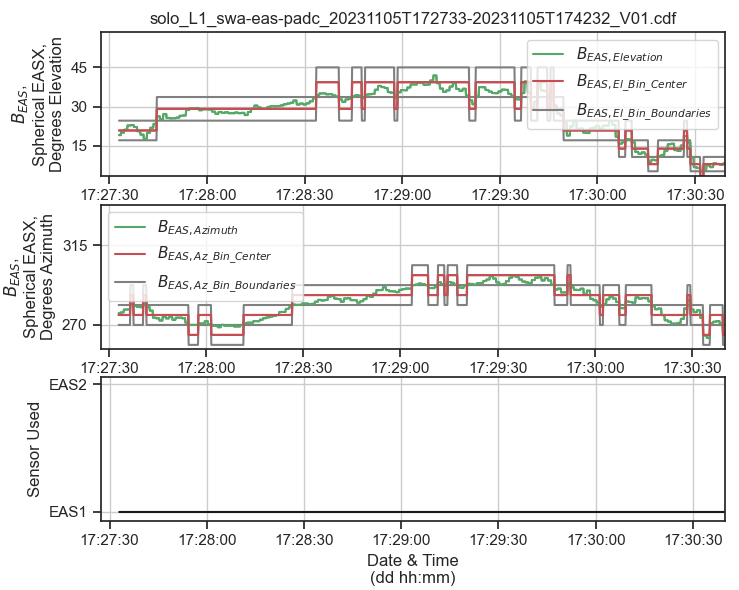
\includegraphics[width=1.05\linewidth]{figures/Steering Example Detail Start.png}
    \caption{A detailed view of the first \(\sim2.5\) minutes of figure \ref{fig: steering example november}. Top panel: Elevation + binning for \(B_{EAS}\) in spherical EASX. Middle panel: Azimuth + binning for \(B_{EAS}\) in spherical EASX. Bottom panel: The selected head over time.}
    \caption*{Image Source: Author's own work}
    \label{fig: steering example november detail}
\end{figure}

To better understand sources of error in Burst Mode data, the Burst Mode steering algorithm was simulated in Python using \(B_{EAS}\) vectors, table \ref{fig: trans example}, and the latest published binning tables shown in appendix \ref{appendixlabel1}. As per section \ref{EAS Burst Mode}, the algorithm first requires a comparison between \(B_{EAS}\) and both EAS head aperture center planes in SRF coordinates, equivalent to their z-axes + 90\degree\ elevation in their respective EAS coordinates. The smallest angle selects the EAS frame to which \(B_{EAS}\) should be transformed. Part of this algorithm is implemented in Python as follows:
\\

[insert code here]
\\

The algorithm then refers to the bin tables and selects the bins corresponding to the elevation and azimuth angles of each vector. This is implemented in Python as follows:
\\

[insert more code here]
\\

The anti-parallel vector to \(B_{EAS}\) is also determined and binned, resulting in two selected elevation bins. 
To validate the simulated binning algorithm, the time series for \(B_{EAS}\) can be plotted against the selected bin centers and upper and lower bounds. If head-selection has been performed correctly, then the \(B_{EAS}\) elevation component should never exceed \(\pm45\degree\). An example of such a plot, showing only the parallel vectors, is shown in figures \ref{fig: steering example november} and \ref{fig: steering example november detail} along with a plot of the chosen head over time, for a 15-minute period on 5th November 2023. Figure \ref{fig: steering example november} shows that the elevation and azimuth values "jump" as the reference frame switches from EAS1 to EAS2 towards the end of the time series. As expected, this switch can be triggered by the \(B_{EAS}\) elevation exceeding \(\pm45\degree\) in its previous head's reference frame. Figure \ref{fig: steering example november detail} provides a detailed view of the algorithm's selection of appropriate binning such that the \(B_{EAS}\) trace stays between bin boundaries.
\\

The most direct way to validate the algorithm is to compare the simulated bins and heads selected to the actual bins and heads selected for a given dataset. EAS level 1 Burst Mode CDF data files on SOAR provide this information. The variable "SWA\_EAS\_EasUsed" contains a time series indicating the head selected (0 for EAS1, 1 for EAS2). "SWA\_EAS\_ElevationUsed" contains a 2D time series with the bin indices (0-15) of the elevation bins selected for parallel and anti-parallel \(B_{EAS}\). "SWA\_EAS\_ELEVATION", "SWA\_EAS\_ELEVATION\_delta\_lower", and "SWA\_EAS\_ELEVATION\_delta\_upper" contain 2D time series with the actual bin centers and boundaries for the selected elevation bins (in degrees), for parallel and anti-parallel \(B_{EAS}\), and likewise for azimuth bins with "SWA\_EAS\_AZIMUTH", "SWA\_EAS\_AZIMUTH\_delta\_lower", and "SWA\_EAS\_AZIMUTH\_delta\_upper" respectively.


\section{EAS Bin Visualisation}
To facilitate the determination of Burst Mode data accuracy, a visualisation tool was developed for this project based on a plot produced by Owen et al for their 2021 publication\cite{owen2021}. This was the tool that was used to create figures \ref{fig: all bins}, \ref{fig: normal - full contours}, and \ref{fig: normal - full contours + selection} in section \ref{EAS PAD}. This visualisation is attractive because it concisely displays magnetic field vectors in SRF, circumventing the need to change coordinates following a sensor head change. The choice of SRF over RTN has been justified in section \ref{coordinate systems}. This visualisation also allows the difference in angular bin widths to be seen projected on to the sky, visualising each head and pixel's field of view along with the ensuing effects on Burst Mode steering.
\\

The visualisation was implemented in Python. The first step was to plot the grid of angular EAS bins in SRF space. Plotting the grid is easily (though inefficiently) accomplished in the EAS1/2 frame using spherical coordinates by simply plotting many closely-spaced points in straight lines along the upper and lower bounds of the elevation and azimuth bin tables (appendix \ref{appendixlabel1}). A single elevation bin can be defined by keeping the elevation angle of successive points constant (and equal to an upper/lower bound) while the azimuth phase angle is varied according to a defined angular point density, and vice versa for a single azimuth bin. Repeating this for the upper and lower edge of an elevation bin and an azimuth bin defines an elevation-azimuth pixel. Once defined, the points of each pixel can be projected to SRF space in spherical coordinates with the following sequence of transformations: Spherical EAS1/2 \(\rightarrow\) Cartesian EAS1/2 \(\rightarrow\) Cartesian SRF \(\rightarrow\) Spherical SRF. This pixel point plotting algorithm was implemented in Python as follows:
\\

\lstset{basicstyle=\tiny, style=myCustomMatlabStyle}
\begin{lstlisting}[language=Python]
angleStep = 1/pointDensity
azimuthPointCount = int(pointDensity*360/azimBinCount)
for i in range(elevBinCount):
    elevationBinWidth = 2*elevDeltaLowerArray[i]
    elevationPointCount = int(point_density*elevationBinWidth)
    binBoundaryProjectionArray.append([])
    for j in range(azimBinCount):
        pointArray = []
        for k_az in range(0,azimuthPointCount):
            lowerEdge_elev = np.array([1, elevLowerBoundArray[i], azimLowerBoundArray[j]+k_az*angleStep])
            lowerEdge_elev = cartToSphere(cart_proj_tuple[head].dot(sphereToCart(lowerEdge_elev)))
            pointArray.append(lowerEdge_elev)

            upperEdge_elev = np.array([1, elevUpperBoundArray[i], azimLowerBoundArray[j]+k_az*angleStep])
            upperEdge_elev = cartToSphere(cart_proj_tuple[head].dot(sphereToCart(upperEdge_elev)))
            pointArray.append(upperEdge_elev)

        for k_el in range(0,elevationPointCount):
            lowerEdge_azim = np.array([1, elevLowerBoundArray[i]+k_el*angleStep, azimLowerBoundArray[j]])
            lowerEdge_azim = cartToSphere(cart_proj_tuple[head].dot(sphereToCart(lowerEdge_azim)))
            pointArray.append(lowerEdge_azim)

            upperEdge_azim = np.array([1, elevLowerBoundArray[i]+k_el*angleStep, azimUpperBoundArray[j]])
            upperEdge_azim = cartToSphere(cart_proj_tuple[head].dot(sphereToCart(upperEdge_azim)))
            pointArray.append(upperEdge_azim)
\end{lstlisting}
\\

where k\_az and k\_el represent integer numbers of azimuth and elevation phase angles along a single bin edge respectively. This algorithm double-counts edges shared between adjacent pixels, trading a linear amount of computational efficiency for some convenience in plotting individual pixels. Once the points are transformed to spherical SRF coordinates, their azimuth angles are converted from the range (-180,180] to the range (0,360] for uniformity with EAS azimuth conventions. Given sufficient point density (20/\degree\ works well), this results in the mostly-continuous, visually-curved bins shown in figure \ref{fig: all bins}. Another result of high point density is that this algorithm's many matrix multiplications for each point transformation lead to a computation time of several minutes for a single image. To save time, the algorithm was adapted to save the point coordinates for each pixel to .csv files in a directory under "bin\_projections\(\backslash\)EAS\textit{X}\(\backslash\)el\textit{Y}\(\backslash\)EAS\textit{X}\_el\textit{Y}\_az\textit{Z}.csv" where \textit{X} is the EAS head number and \textit{Y} and \textit{Z} are the elevation and azimuth bin indices respectively. These files can then be read and plotted with an order of magnitude reduction in computation time. This was essentially implemented in Python as follows:
\newpage
\lstset{basicstyle=\tiny, style=myCustomMatlabStyle}
\begin{lstlisting}[language=Python]
for i in range(16):
        for j in range(32):
                filename = 'bin_projections\EAS{head}\el{i}\EAS{head}_el{i}_az{j}.csv'
                pixelArray = np.genfromtxt(filename, delimiter=",")
                el = pixelArray[1]
                az = pixelArray[2]
                ax.scatter(az,el,color=bin_color,marker='.',s=s)
\end{lstlisting}
\\

Plotting the parallel and antiparallel magnetic field vectors seen in figures \ref{fig: normal - full contours} and \ref{fig: normal - full contours + selection} was relatively simple. Since both \(B_{EAS}\) and \(B_{MAG}\) are acquired from SOAR in SRF coordinates, they only had to be transformed to spherical coordinates and plotted. To plot the contours of constant pitch angle at arbitrary pitch angles around these vectors, involved an adaptation of an algorithm written by Chris Owen in Interactive Data Language (IDL)\cite{owen2021}. The algorithm starts by constructing the cartesian transformation matrix \textit{M} from a reference frame whose z-axis is aligned with the magnetic field vector to SRF coordinates. \textit{M} is constructed as shown in table \ref{tab: Matrix M}.

\begin{table}[h!]
    \centering
    \(M=
    \begin{bmatrix}
    \cos{\phi}\cos{\theta} & \sin{\phi}\cos{\theta} & \sin{\theta}\\
    -\sin{\phi} & \cos{\phi} & 0\\
    -\cos{\phi}\sin{\theta} & -\sin{\phi}\sin{\theta} & \cos{\theta}\\
    \end{bmatrix} &
    \)\\
    \caption{The matrix \textit{M} transforming a spherical SRF vector with \(\theta=\textrm{elevation}*\pi/180\degree\) and \(\phi=\textrm{azimuth}*\pi/180\degree\) into a cartesian, field-aligned reference frame.} 
    \label{tab: Matrix M}
\end{table}
\\

From there, the the proceeding algorithm can be summarised as follows:
\begin{enumerate}
    \item 
    \item 
    \item 
\end{enumerate}

\section{Completeness Algorithm}
Research into the steering algorithm and data visualisation completed earlier in this project made it clear that there is a relatively fast approach to generating a "completeness" or "quality" score for Burst Mode PADs, circumventing the relatively expensive process of rebinning EAS Burst Mode VDF data to generate the PADs in the first place, and then assessing PAD completeness "by hand" (e.g. by counting the white bins in figure \ref{PAD example}).\\

While the binning issue described in section \ref{sim steering} affects PAD completeness, its effects are expected to be completely captured by the completeness algorithm as-is. The binning issue concerns the discrepancy between \(B_{EAS}\) and its selected bins, while the completeness algorithm concerns the discrepancy between \(B_{MAG}\) and the selected elevation bins. Whether or not these elevation bins were selected correctly only indirectly affects the completeness score depending on the agreement between \(B_{EAS}\) and \(B_{MAG}\). In fact, given sufficient disagreement between \(B_{EAS}\) and \(B_{MAG}\), the binning issue may lead \(B_{MAG}\) to be binned \textit{more accurately} than \(B_{EAS}\) (for example, if \(B_{EAS}\) is binned incorrectly while \(B_{MAG}\), by chance, is binned correctly).
\\

\blindtext

\section{S20 Link Latency}
It is possible that some of the \(B_{EAS}\)-\(B_{MAG}\) discrepancy can be attributed to latency over the S20 inter-instrument data link\cite{owen2021}.  This latency may be particularly noticeable on 1/8th second timeframe during periods of heavy data traffic\cite{owen2021}. If noticeable, then the latency is expected to cause a time delay between \(B_{EAS}\) and \(B_{MAG}\) where \(B_{MAG}\) leads by at least \(\sim\)0.125s. One approach to measuring this time delay is to perform a cross-correlation analysis between \(B_{EAS}\) and \(B_{MAG}\)\cite{hanus2019}); in principle, a cross-correlation function (CCF) takes a domain of time delays as input and the delay that gives the strongest correlation between the two time series can be selected to represent the latency. The principle behind this approach is well-illustrated by figure \ref{fig: Hanus CCF} by Hanus et al\cite{hanus2019} for two 1D time series \(x(t)\) and \(z(t)\) and latency \(\tau_0\).

\begin{figure}[h!]
    \centering
    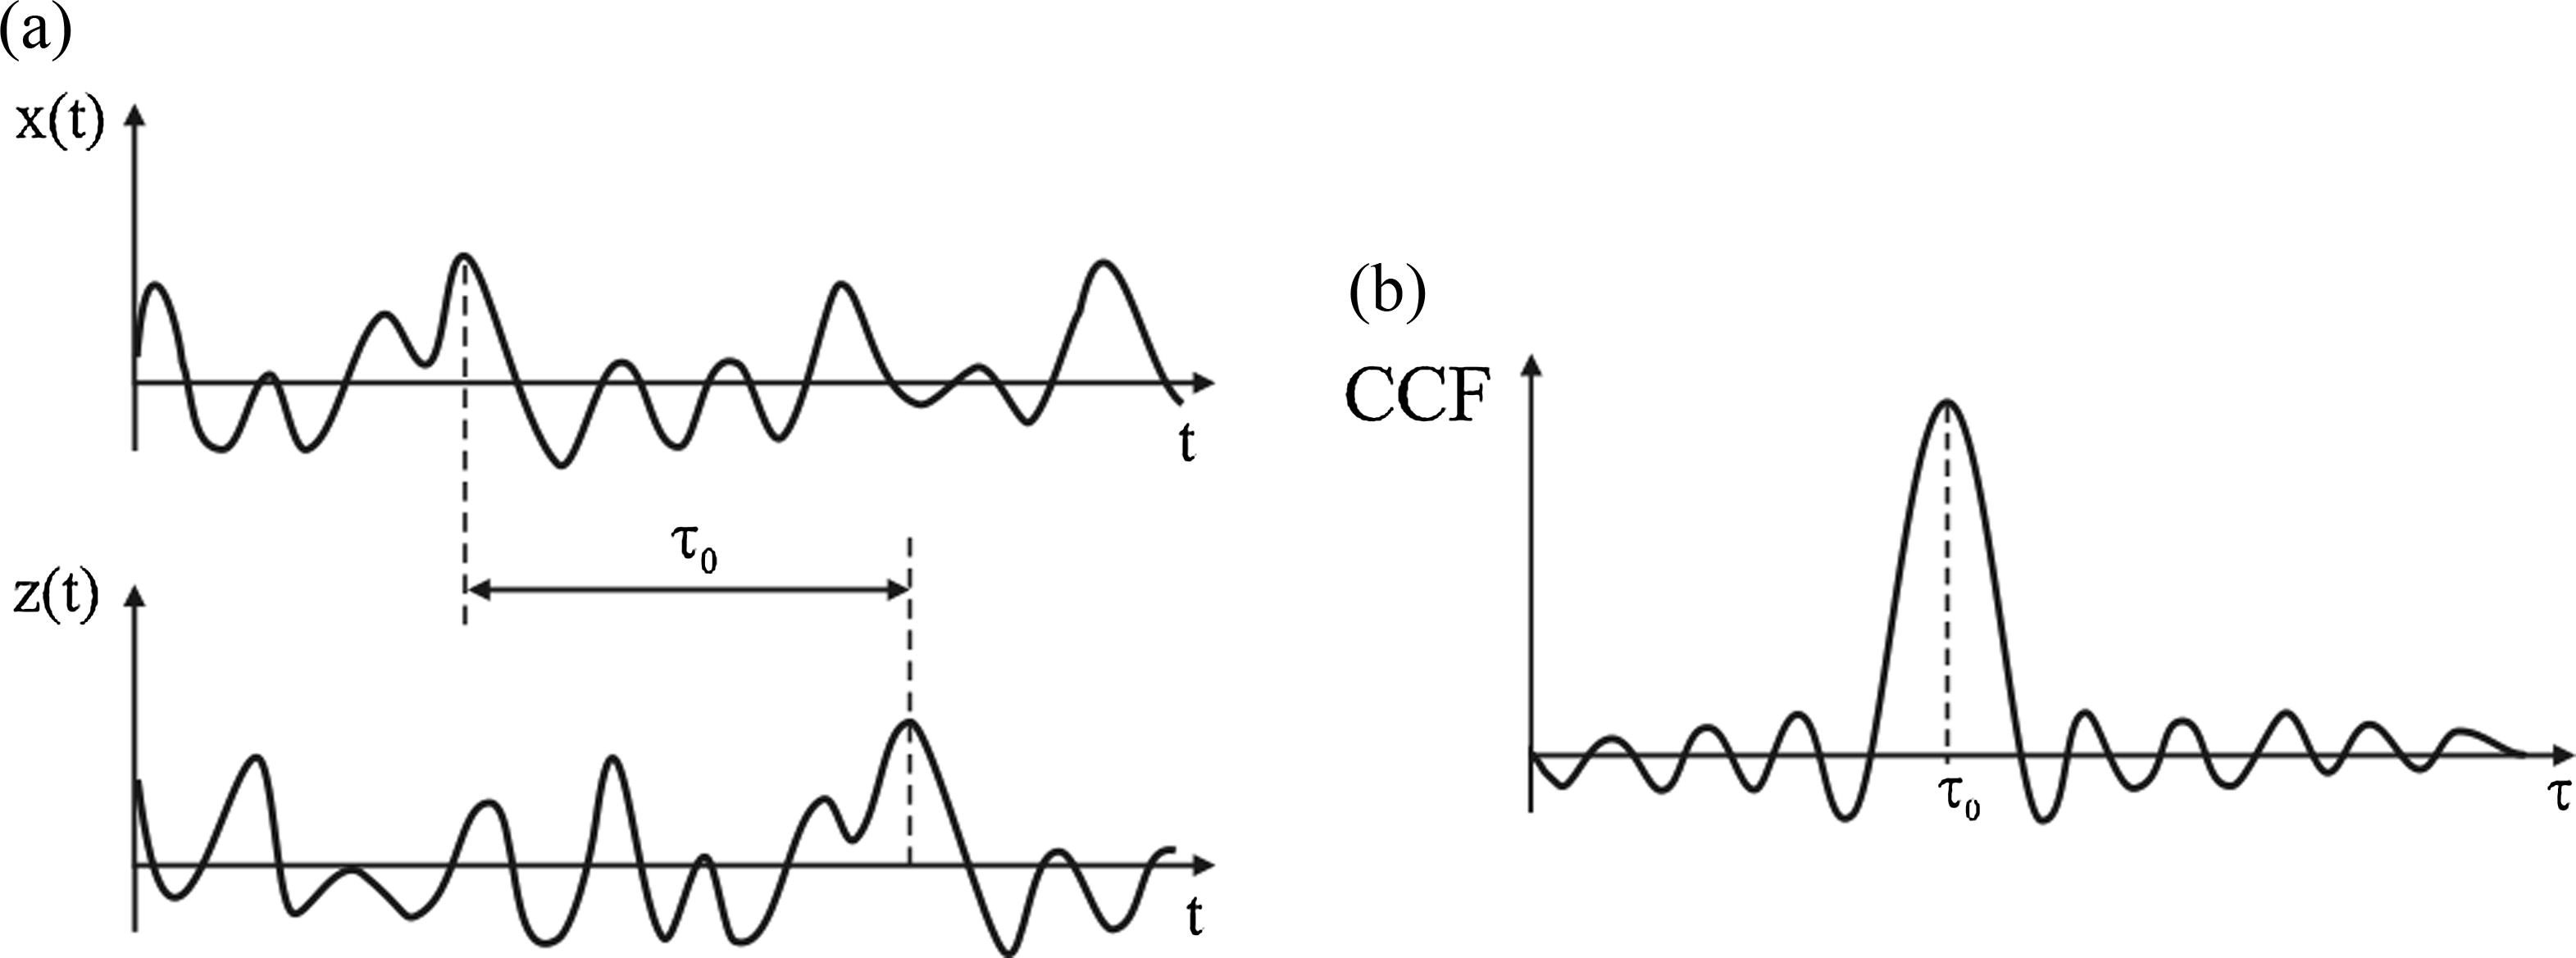
\includegraphics[width=1\linewidth]{figures/hanus diagram.jpg}
    \caption{Two figures illustrating CCF time delay determination. (a): Two arbitrary time series \(x(t)\) and \(z(t)\), which are well-approximated as identical time series with a time delay \(\tau_0\) between them. (b): A plot of the CCF applied to \(x(t)\) and \(z(t)\), showing maximum correlation at the time delay \(\tau_0\), representing the latency.}
    \caption*{Image Source: Hanus et al\cite{hanus2019}}
    \label{fig: Hanus CCF}
\end{figure}

\blindtext


\chapter{Results and Analysis}
\label{chapterlabel3}

% This just dumps some pseudolatin in so you can see some text in place.
\blindtext

\section{Time Series Comparison}
\blindtext

\section{Completeness}
\blindtext

\section{S20 Link Latency}
\blindtext

\section{SWA-DPU Binning Error}
\blindtext
\chapter{Conclusion}
\label{chapterlabel4}

% This just dumps some pseudolatin in so you can see some text in place.
\blindtext
\phantomsection
\addcontentsline{toc}{chapter}{Appendices}

% The \appendix command resets the chapter counter, and changes the chapter numbering scheme to capital letters.
%\chapter{Appendices}
\appendix
\chapter{EAS Head Angular Bin Widths}
\label{appendixlabel1}

\begin{table}[h]
    \centering
    \centerfloat
    \begin{tabular}{cccc}
        \textbf{EAS1/2 Bin Index} & \textbf{Bin Center (\degree)} & \textbf{Bin Upper Delta (\degree)} & \textbf{Bin Lower Delta (\degree)}\\
        0 & 5.625 & 5.625 & 5.625\\
        1 & 16.875 & 5.625 & 5.625\\
        2 & 28.125 & 5.625 & 5.625\\
        3 & 39.375 & 5.625 & 5.625\\
        4 & 50.625 & 5.625 & 5.625\\
        5 & 61.875 & 5.625 & 5.625\\
        6 & 73.125 & 5.625 & 5.625\\
        7 & 84.375 & 5.625 & 5.625\\
        8 & 95.625 & 5.625 & 5.625\\
        9 & 106.875 & 5.625 & 5.625\\
        10 & 118.125 & 5.625 & 5.625\\
        11 & 129.375 & 5.625 & 5.625\\
        12 & 140.625 & 5.625 & 5.625\\
        13 & 151.875 & 5.625 & 5.625\\
        14 & 163.125 & 5.625 & 5.625\\
        15 & 174.375 & 5.625 & 5.625\\
        16 & 185.625 & 5.625 & 5.625\\
        17 & 196.875 & 5.625 & 5.625\\
        18 & 208.125 & 5.625 & 5.625\\
        19 & 219.375 & 5.625 & 5.625\\
        20 & 230.625 & 5.625 & 5.625\\
        21 & 241.875 & 5.625 & 5.625\\
        22 & 253.125 & 5.625 & 5.625\\
        23 & 264.375 & 5.625 & 5.625\\
        24 & 275.625 & 5.625 & 5.625\\
        25 & 286.875 & 5.625 & 5.625\\
        26 & 298.125 & 5.625 & 5.625\\
        27 & 309.375 & 5.625 & 5.625\\
        28 & 320.625 & 5.625 & 5.625\\
        29 & 331.875 & 5.625 & 5.625\\
        30 & 343.125 & 5.625 & 5.625\\
        31 & 354.375 & 5.625 & 5.625\\
    \end{tabular}
    \caption{Bin Table: EAS1/2 Azimuth - 17th July 2021}
    \label{tab: Bin Table EAS Azimuth July 2021}
\end{table}

\begin{table}[h]
    \centering
    \centerfloat
    \begin{tabular}{cccc}
        \textbf{EAS1 Bin Index} & \textbf{Bin Center (\degree)} & \textbf{Bin Upper Delta (\degree)} & \textbf{Bin Lower Delta (\degree)}\\
        0 & 39.34 & 5.66 & 5.66\\
        1 & 29.17 & 4.514 & 4.514\\
        2 & 20.91 & 3.748 & 3.748\\
        3 & 13.98 & 3.179 & 3.179\\
        4 & 8.06 & 2.74 & 2.74\\
        5 & 2.91 & 2.409 & 2.409\\
        6 & -1.66 & 2.161 & 2.161\\
        7 & -5.82 & 1.996 & 1.996\\
        8 & -9.7 & 1.886 & 1.886\\
        9 & -13.43 & 1.841 & 1.841\\
        10 & -17.13 & 1.856 & 1.856\\
        11 & -20.94 & 1.95 & 1.95\\
        12 & -25.0 & 2.115 & 2.115\\
        13 & -29.53 & 2.413 & 2.413\\
        14 & -34.82 & 2.88 & 2.88\\
        15 & -41.36 & 3.655 & 3.655\\
    \end{tabular}
    \caption{Bin Table: EAS1 Elevation - 17th July 2021}
    \label{tab: Bin Table EAS1 Elevation July 2021}
\end{table}

\begin{table}[h]
    \centering
    \centerfloat
    \begin{tabular}{cccc}
        \textbf{EAS2 Bin Index} & \textbf{Bin Center (\degree)} & \textbf{Bin Upper Delta (\degree)} & \textbf{Bin Lower Delta (\degree)}\\
        0 & 38.94 & 6.06 & 6.06\\
        1 & 28.25 & 4.633 & 4.633\\
        2 & 19.86 & 3.761 & 3.761\\
        3 & 12.99 & 3.111 & 3.111\\
        4 & 7.25 & 2.624 & 2.624\\
        5 & 2.35 & 2.272 & 2.272\\
        6 & -1.93 & 2.012 & 2.012\\
        7 & -5.78 & 1.838 & 1.838\\
        8 & -9.37 & 1.747 & 1.747\\
        9 & -12.84 & 1.722 & 1.722\\
        10 & -16.32 & 1.759 & 1.759\\
        11 & -19.97 & 1.887 & 1.887\\
        12 & -23.97 & 2.113 & 2.113\\
        13 & -28.57 & 2.485 & 2.485\\
        14 & -34.13 & 3.071 & 3.071\\
        15 & -41.1 & 3.897 & 3.897\\
    \end{tabular}
    \caption{Bin Table: EAS2 Elevation - 17th July 2021}
    \label{tab: Bin Table EAS2 Elevation July 2021}
\end{table}

\chapter{Another Appendix About Things}
\label{appendixlabel2}
(things)

\chapter{Colophon}
\label{appendixlabel3}
\textit{This is a description of the tools you used to make your thesis. It helps people make future documents, reminds you, and looks good.}

\textit{(example)} This document was set in the Times Roman typeface using \LaTeX\ and Bib\TeX , composed with a text editor. 
 % description of document, e.g. type faces, TeX used, TeXmaker, packages and things used for figures. Like a computational details section.
% e.g. http://tex.stackexchange.com/questions/63468/what-is-best-way-to-mention-that-a-document-has-been-typeset-with-tex#63503

% Side note:
%http://tex.stackexchange.com/questions/1319/showcase-of-beautiful-typography-done-in-tex-friends
 
% You could separate these out into different files if you have
%  particularly large appendices.

% Actually generates your bibliography. The fact that \include is 
% the last thing before this ensures that it is on a clear page.
\bibliography{citations}

% All done. \o/
\end{document}
